% ===== CHATPTER 7 =====
\chapter{量子力学理论}
\label{chap:7}
\section{符号}
\label{sec:7.1 Notation}
    单电子原子的薛定谔方程(第\ref{chap:6}章)是可以精确求解的。然而,由于哈密顿算符中的电子间斥力项,多电子原子和分子的薛定谔方程无法精确求解。因此,我们必须寻求近似的求解方法。第 \ref{chap:8} 章和第 \ref{chap:9} 章将介绍两种主要的近似方法,即变分法和微扰理论。要推导出这些方法,我们必须进一步发展量子力学理论,这就是本章所要做的。

    在开始之前,我们先介绍一些符号。夹在两个函数之间的算符在全空间上的定积分经常出现,并使用各种缩写:
    \begin{equation}
        \int f^{\ast}_m\hat{A}f_n\mathrm{d}\tau \equiv \left\langle f_m \middle| \hat{A} \middle| f_n \right\rangle \equiv \left\langle m \middle| \hat{A} \middle| n \right\rangle
        \label{eq:7.1}
    \end{equation}
    其中$f_m$和$f_n$是两个函数。如式(\ref{eq:7.1})所示,若两个函数的含义是明确的,我们就可以只用下标来区分。狄拉克引入的上述符号称为\textbf{括号符号}(bracket notation)(此处为直译,多用狄拉克符号,下同)。另一种符号是
    \begin{equation}
        \int f^{\ast}_m\hat{A}f_n\mathrm{d}\tau \equiv A_{mn}
        \label{eq:7.2}
    \end{equation}
    符号$A_{mn}$和$\left\langle m \middle| \hat{A} \middle| n \right\rangle$都表示我们使用字母在前的复函数的复共轭。定积分$\left\langle m \middle| \hat{A} \middle| n \right\rangle$称为算符$\hat{A}$的一个\textbf{矩阵元}(matrix element)。矩阵是数字的矩形数组,遵守一定的组合规则(见第 \ref{sec:7.10 Matrices} 节)。

    我们将对两个函数全空间的定积分写作
    \begin{equation}
        \int f^{\ast}_m f_n \mathrm{d}\tau \equiv \left\langle f_m \middle| f_n \right\rangle \equiv \left\langle m \middle| n \right\rangle
        \label{eq:7.3}
    \end{equation}
    注意:
    \begin{equation*}
        \left\langle f \middle| \hat{B} \middle| g \right\rangle = \left\langle f \middle| \hat{B} g \right\rangle
    \end{equation*}
    其中$f$和$g$是函数。由于$\left(\int f^{\ast}_mf_n\mathrm{d}\tau\right)^{\ast} = \int f^{\ast}_nf_m\mathrm{d}\tau$,我们可以得到
    \begin{equation}
        \boxed{
            \left\langle m \middle| n \right\rangle^{\ast} = \left\langle n \middle| m \right\rangle
        }
        \label{eq:7.4}
    \end{equation}
    由于取了 (\ref{eq:7.1}) 中 $f_m$ 的复共轭,因此可以得出
    \begin{equation}
        \boxed{
            \left\langle cf \middle| \hat{B} \middle| g \right\rangle = c^{\ast} \left\langle f \middle| \hat{B} \middle| g \right\rangle \quad \text{和} \quad \left\langle f \middle| \hat{B} \middle| cg \right\rangle = c \left\langle f \middle| \hat{B} \middle| g \right\rangle
        }
        \label{eq:7.5}
    \end{equation}
    其中$\hat{B}$是线性算符,$c$是常数。

\section{厄米算符}
\label{sec:7.2 Hermitian Operators}
    代表物理量的量子力学算符都是线性算符(第\ref{sec:3.1 Operators}节)。这些算符必须满足一个额外的要求,我们现在就来讨论这个问题。

\subsection*{厄米算符的定义}

    设$\hat{A}$是对应某个物理量$A$的线性算符。则$A$的平均期望为[式(\ref{eq:3.88})]
    \begin{equation*}
        \left\langle A \right\rangle = \int \Psi^{\ast} \hat{A} \Psi \mathrm{d}\tau
    \end{equation*}
    其中$\Psi$是系统的态函数。由于物理量的平均值一定是一个实数,我们要求
    \begin{equation*}
        \left\langle A \right\rangle = \left\langle A \right\rangle^{\ast}
    \end{equation*}
    \begin{equation*}
        \int \Psi^{\ast} \hat{A} \Psi \mathrm{d}\tau = \left[\int \Psi^{\ast}\hat{A}\Psi\mathrm{d}\tau\right] = \int \left(\Psi^{\ast}\right)^{\ast} \left(\hat{A}\Psi\right)^{\ast}\mathrm{d}\tau
    \end{equation*}
    \begin{equation}
        \int \Psi^{\ast} \hat{A} \Psi \mathrm{d}\tau = \int \Psi  \left(\hat{A}\Psi\right)^{\ast} \mathrm{d}\tau
        \label{eq:7.6}
    \end{equation}
    式(\ref{eq:7.6})必须对每个代表系统可能状态的波函数$\Psi$都成立,也就是说,所有品优函数$\Psi$都必须满足式(\ref{eq:7.6})。对所有品优函数都满足式(\ref{eq:7.6})的算符称为\textbf{厄米算符}(Hermitian operator)(由数学家厄米的名字命名——Charles Hermite)。

    许多教科书将厄米算符定义为对所有品优函数$f$和$g$都满足下式的线性算符:
    \begin{equation}
        \int f^{\ast} \hat{A} g \:\mathrm{d}\tau = \int g \:\left(\hat{A} f\right)^{\ast} \mathrm{d}\tau
        \label{eq:7.7}
    \end{equation}
    注意:在(\ref{eq:7.7})的左侧,算符$\hat{A}$作用在函数$g$上;而在右侧,算符$\hat{A}$作用在函数$f$上。对于特例$f=g$,式(\ref{eq:7.7})退化为式(\ref{eq:7.6})。等式 (\ref{eq:7.7}) 显然是比 (\ref{eq:7.6}) 更强的要求,但我们将证明 (\ref{eq:7.7}) 是 (\ref{eq:7.6}) 的结果。因此,两种厄米算符的定义是等价的。

    我们首先在 (\ref{eq:7.6}) 中令 $ \Psi = f+cg$ ,其中 $c$ 是一个任意常数。则
    \begin{equation*}
        \int \left(f+cg\right)^{\ast}\hat{A}\left(f+cg\right)\mathrm{d}\tau = \int \left(f+cg\right)\left[\hat{A}\left(f+cg\right)\right]^{\ast}\mathrm{d}\tau
    \end{equation*}
    \begin{equation*}
        \begin{aligned}
            \int \left(f^{\ast}+c^{\ast}g^{\ast}\right)\hat{A}f\mathrm{d}\tau + \int \left(f^{\ast} +c^{\ast}g^{\ast} \right)&\hat{A}cg \:\mathrm{d}\tau \\
            & = \int \left(f+c g\right)\left(\hat{A}f\right)^{\ast} \mathrm{d}\tau + \int \left(f+c g\right)\left(\hat{A}cg\right)^{\ast} \mathrm{d}\tau
        \end{aligned}
    \end{equation*}
    \begin{equation*}
        \begin{aligned}
            \int f^{\ast} \hat{A} f \:\mathrm{d}\tau + & c^{\ast} \int g^{\ast} \hat{A} f \:\mathrm{d}\tau + c \int f^{\ast} \hat{A} g \:\mathrm{d}\tau + c^{\ast}c \int g^{\ast} \hat{A} g \:\mathrm{d}\tau  \\
            & =\int f \left(\hat{A}f\right)^{\ast} \mathrm{d}\tau + c \int g \left(\hat{A}f\right)^{\ast} \mathrm{d}\tau + c^{\ast} \int f \left(\hat{A}g\right)^{\ast} \mathrm{d}\tau + cc^{\ast}\int g \left(\hat{A}g\right)^{\ast} \mathrm{d}\tau
        \end{aligned}
    \end{equation*}
    根据 (\ref{eq:7.6}),最后一个等式两边的首项相等;同样,两边的尾项也相等。因此,
    \begin{equation}
        c^{\ast} \int g^{\ast} \hat{A} f \:\mathrm{d}\tau + c \int f^{\ast} \hat{A} g \:\mathrm{d}\tau = c \int g \left(\hat{A}f\right)^{\ast} \mathrm{d}\tau + c^{\ast} \int f \left(\hat{A}g\right)^{\ast} \mathrm{d}\tau
        \label{eq:7.8}
    \end{equation}
    在(\ref{eq:7.8})中令$c=1$,我们有
    \begin{equation}
        \int g^{\ast} \hat{A} f \:\mathrm{d}\tau + \int f^{\ast} \hat{A} g \:\mathrm{d}\tau = \int g \left(\hat{A}f\right)^{\ast} \mathrm{d}\tau + \int f \left(\hat{A}g\right)^{\ast} \mathrm{d}\tau
        \label{eq:7.9}
    \end{equation}
    在(\ref{eq:7.8})中令$c = \mathrm{i}$,两边同除以$\mathrm{i}$,我们有
    \begin{equation}
        - \int g^{\ast} \hat{A} f \:\mathrm{d}\tau + \int f^{\ast} \hat{A} g \:\mathrm{d}\tau = \int g \left(\hat{A}f\right)^{\ast} \mathrm{d}\tau - \int f \left(\hat{A}g\right)^{\ast} \mathrm{d}\tau
        \label{eq:7.10}
    \end{equation}
    将(\ref{eq:7.9})和(\ref{eq:7.10})相加,我们得到了(\ref{eq:7.7})。结论得到了证明。

    因此,\textit{厄米算符$\hat{A}$定义为满足如下条件的线性算符:}
    \begin{equation}
        \boxed{
            \int f^{\ast}_m \hat{A} f_n \:\mathrm{d}\tau = \int f_n \left(\hat{A} f_m\right)^{\ast} \mathrm{d}\tau
        }
        \label{eq:7.11}
    \end{equation}
    \textit{其中$f_m$和$f_n$是任意的品优函数,积分为对全空间的定积分。}使用狄拉克符号和矩阵元符号,我们将其记作
    \begin{equation}
        \boxed{
            \left\langle f_m \middle| \hat{A} \middle| f_n \right\rangle = \left\langle f_n \middle| \hat{A} \middle| f_m \right\rangle^{\ast}
        }
        \label{eq:7.12}
    \end{equation}
    \begin{equation}
        \boxed{
            \left\langle m \middle| \hat{A} \middle| n \right\rangle = \left\langle n \middle| \hat{A} \middle| m \right\rangle^{\ast}
        }
        \label{eq:7.13}
    \end{equation}
    \begin{equation}
        \boxed{
            A_{mn} = \left(A_{nm}\right)^{\ast}
        }
        \label{eq:7.14}
    \end{equation}
    (\ref{eq:7.12}) 的两边不同之处在于交换了函数并取了复共轭。

\subsection*{厄米算符的例子}

    让我们证明,我们一直在使用的一些算符确实是厄米的。简单起见,我们将从一个维度进行研究。要证明一个算符是厄米的,只需证明它对所有品优函数都满足式(\ref{eq:7.6})即可。不过,我们将通过证明满足 (\ref{eq:7.11}) 来增加一点难度。

    首先,来考虑单粒子一维势能算符。式(\ref{eq:7.11})的右侧为
    \begin{equation}
        \int_{-\infty}^{\infty} f_n\left(x\right)\left[V\left(x\right)f_m\left(x\right)\right]^{\ast} \mathrm{d}x
        \label{eq:7.15}
    \end{equation}
    由于势能是实函数,我们有$V^{\ast} = V$。此外,式(\ref{eq:7.15})中因子的顺序无关紧要。因此,
    \begin{equation*}
        \int_{-\infty}^{\infty} f_n\left(Vf_m\right)^{\ast} \mathrm{d}x = \int_{-\infty}^{\infty} f_n V^{\ast} f^{\ast}_m \mathrm{d}x = \int_{-\infty}^{\infty} f_m^{\ast} V f_n \mathrm{d}x
    \end{equation*}
    这就证明了$V$是厄米的。

    再考虑动量在$x$方向分量的算符$\hat{p}_x = -\mathrm{i}\hbar \: \mathrm{d}/\mathrm{d}x$[式(\ref{eq:3.23})]。对于这个算符,式(\ref{eq:7.11})的左侧为
    \begin{equation*}
        -\mathrm{i}\hbar \int_{-\infty}^{\infty} f_m^{\ast}\left(x\right)\frac{\mathrm{d}f_n\left(x\right)}{\mathrm{d}x} \mathrm{d}x
    \end{equation*}
    现在我们使用分部积分法:
    \begin{equation}
        \int_{a}^{b}u\left(x\right)\frac{\mathrm{d}v\left(x\right)}{\mathrm{d}x}\mathrm{d}x = \left. u\left(x\right)v\left(x\right)\right|_{a}^{b} - \int_{a}^{b}v\left(x\right)\frac{\mathrm{d}u\left(x\right)}{\mathrm{d}x}\mathrm{d}x
        \label{eq:7.16}
    \end{equation}
    令
    \begin{equation*}
        u\left(x\right) \equiv -\mathrm{i}\hbar f_m^{\ast}\left(x\right), \quad v\left(x\right) \equiv f_n\left(x\right)
    \end{equation*}
    那么
    \begin{equation}
        -\mathrm{i}\hbar f_m^{\ast}\frac{\mathrm{d}f_n}{\mathrm{d}x}\mathrm{d}x = \left. -\mathrm{i}\hbar f_m^{\ast}f_n\right|_{-\infty}^{\infty} + \mathrm{i}\hbar \int_{-\infty}^{\infty} f_n\left(x\right)\frac{\mathrm{d}f_m^{\ast}\left(x\right)}{\mathrm{d}x}\mathrm{d}x
        \label{eq:7.17}
    \end{equation}
    由于$f_m$和$f_n$是品优函数,因此在无穷远处它们的值为(如果它们在无穷远处不为零,则不符合平方可积的要求)。于是,(\ref{eq:7.17})变为
    \begin{equation*}
        \int_{-\infty}^{\infty} f_m^{\ast}\left(-\mathrm{i}\hbar \frac{\mathrm{d}f_n}{\mathrm{d}x}\right)\mathrm{d}x = \int_{-\infty}^{\infty} f_n\left(-\mathrm{i}\hbar \frac{\mathrm{d}f_m}{\mathrm{d}x}\right)^{\ast}\mathrm{d}x
    \end{equation*}
    与(\ref{eq:7.11})一致,证明了$\hat{p}_x$是厄米的。证明动能算符是厄米的留给读者自行考虑。可以证明,两个厄米算符的和也是厄米的。因此,哈密顿算符$\hat{H} = \hat{T} + \hat{V}$也是厄米的。

\subsection*{厄米算符定理}

    现在我们证明一些有关厄米算符的本征值和本征函数的重要定理。

    由于与物理量 $A$ 相对应的算符 $\hat{A}$ 的本征值是测量 $A$ 的可能结果(第 \ref{sec:3.3 Operators and Quantum Mechanics} 节),因此这些特征值都应该是实数。我们现在证明厄米算符的本征值是实数。

    我们现在知道$\hat{A}$是厄米算符。将这个条件转换为方程,对于所有品优函数$f_m$和$f_n$,我们有[式(\ref{eq:7.11})]
    \begin{equation}
        \int f^{\ast}_m \hat{A} f_n \:\mathrm{d}\tau = \int f_n \left(\hat{A} f_m\right)^{\ast} \mathrm{d}\tau
        \label{eq:7.18}
    \end{equation}
    我们希望证明$\hat{A}$的每个本征值都是实数。将其转换为方程,我们希望证明$a_i = a_i^{\ast}$,其中本征值$a_i$满足$\hat{A}g_i = a_i g_i$,其中$g_i$是$\hat{A}$的本征函数。

    为了将本征值$a_i$引入式(\ref{eq:7.18}),我们将(\ref{eq:7.18})写成一个特例,其中$f_m = g_i$和$f_n = g_i$:
    \begin{equation*}
        \int g_i^{\ast} \hat{A} g_i \:\mathrm{d}\tau = \int g_i \left(\hat{A} g_i\right)^{\ast} \mathrm{d}\tau
    \end{equation*}
    使用$\hat{A} g_i = a_i g_i$,我们有
    \begin{equation*}
        a_i \int g_i^{\ast} g_i \:\mathrm{d}\tau = \int g_i \left(a_i g_i\right)^{\ast} \mathrm{d}\tau = a_i^{\ast} \int g_i g_i^{\ast} \:\mathrm{d}\tau
    \end{equation*}
    \begin{equation}
        \left(a_i - a_i^{\ast}\right) \int \left|g_i\right|^2 \:\mathrm{d}\tau = 0
        \label{eq:7.19}
    \end{equation}
    由于对$\left|g_i\right|^2$的积分永远不会为负,因此 (\ref{eq:7.19}) 中积分为零的唯一可能情况是 $g_i$ 在所有坐标值下都为零。然而,基于物理原因,我们总是拒绝将 $g_i=0$ 作为本征函数。因此,式(\ref{eq:7.19})中的积分不能为零。那么只有$\left(a_i - a_i^{\ast}\right) = 0$,即$a_i = a_i^{\ast}$。得证。

    \begin{center}
        \parbox{0.8\textwidth}{
            \textbf{定理1:} 厄米算符的本征值为实数。
        }
    \end{center}

    为了帮助读者熟悉狄拉克符号,我们将使用狄拉克符号重新证明定理1。在式(\ref{eq:7.13})中,令$m=i$以及$n=i$,我们得到了$\left\langle i \middle| \hat{A} \middle| i \right\rangle = \left\langle i \middle| \hat{A} \middle| i \right\rangle^{\ast}$。选择下标为$i$的函数作为$\hat{A}$的本征函数,使用本征方程$\hat{A} g_i = a_i g_i$,我们有$\left\langle i \middle| a_i \middle| i \right\rangle = \left\langle i \middle| a_i \middle| i \right\rangle^{\ast}$。因此,$a_i \left\langle i \middle| i \right\rangle = a_i^{\ast} \left\langle i \middle| i \right\rangle^{\ast} = a_i^{\ast}\left\langle i \middle| i \right\rangle$,则$\left(a_i - a_i^{\ast}\right)\left\langle i \middle| i \right\rangle = 0$。所以$a_i = a_i^{\ast}$,其中我们用到了(\ref{eq:7.4})中$m=n$。

    我们已经证明:两个不同的箱中粒子能量本征函数$\psi_i$和$\psi_j$是正交的,也就是说对$i \neq j$,有$\int_{-\infty}^{\infty}\psi_i^{\ast}\psi_j \mathrm{d}x = 0$[式(\ref{eq:2.26 definition of orthogonal wave functions})]。若两个坐标相同的函数$f_1$和$f_2$满足下式。则它们是\textbf{正交的}(orthogonal):
    \begin{equation}
        \boxed{
            \int f_1^{\ast} f_2 \:\mathrm{d}\tau = 0
        }
        \label{eq:7.20}
    \end{equation}
    其中的积分是对坐标的全空间进行定积分。我们现在证明更一般的结论:\textit{厄米算符的本征函数是或可以被选择为相互正交的。}有
    \begin{equation}
        \hat{B}F = sF, \quad \hat{B}G = tG
        \label{eq:7.21}
    \end{equation}
    其中$F$和$G$是厄米算符$\hat{B}$的两个线性无关的本征函数,我们希望证明
    \begin{equation*}
        \int F^{\ast} G \:\mathrm{d}\tau \equiv \left\langle F \middle| G \right\rangle = 0
    \end{equation*}
    我们从 (\ref{eq:7.12}) 开始,它表达了 $\hat{B}$ 的厄米性质:
    \begin{equation*}
        \left\langle F \middle| \hat{B} \middle| G \right\rangle = \left\langle G \middle| \hat{B} \middle| F \right\rangle^{\ast}
    \end{equation*}
    使用式(\ref{eq:7.21}),我们有
    \begin{equation*}
        \left\langle F \middle| t \middle| G \right\rangle = \left\langle G \middle| s \middle| F \right\rangle^{\ast}
    \end{equation*}
    \begin{equation*}
        t \left\langle F \middle| G \right\rangle = s^{\ast} \left\langle G \middle| F \right\rangle
    \end{equation*}
    由于厄米算符的本征值为实数(定理1),我们有$s^{\ast} = s$。使用$\left\langle G \middle| F \right\rangle = \left\langle F \middle| G \right\rangle^{\ast}$(式(\ref{eq:7.4})),我们得到
    \begin{equation*}
        t \left\langle F \middle| G \right\rangle = s \left\langle F \middle| G \right\rangle
    \end{equation*}
    \begin{equation*}
        \left(t - s\right) \left\langle F \middle| G \right\rangle = 0
    \end{equation*}
    若$s \neq t$,则
    \begin{equation}
        \left\langle F \middle| G \right\rangle = 0
        \label{eq:7.22}
    \end{equation}

    我们已经证明,对应于\textit{不同}本征值的厄米算符的两个本征函数是正交的。现在的问题是:我们能否有两个具有\textit{相同}本征值的独立本征函数?答案是肯定的。在\textit{简并}的情况下,我们有一个以上的本征函数有相同的本征值。因此,只有当厄米算符的两个独立本征函数不对应于一个简并本征值时,我们才能确定它们是正交的。现在我们要证明,在简并的情况下,我们可以\textit{构造}出彼此正交的本征函数。我们将使用第 \ref{sec:3.6 Degeneracy} 节中证明的定理,即任何与简并本征值对应的本征函数线性组合都是具有相同本征值的本征函数。因此,让我们假设 $F$ 和 $G$ 是具有相同本征值的独立本征函数:
    \begin{equation*}
        \hat{B}F = sF, \quad \hat{B}G = sG
    \end{equation*}
    我们对 $F$ 和 $G$ 进行线性组合,形成两个新的本征函数 $g_1$ 和 $g_2$,它们将相互正交。我们选择
    \begin{equation*}
        g_1 \equiv F, \quad g_2 \equiv G + cF
    \end{equation*}
    其中常数 $c$ 的选择是为了确保正交性。我们希望
    \begin{equation*}
        \int g_1^{\ast} g_2 \:\mathrm{d}\tau = 0
    \end{equation*}
    \begin{equation*}
        \int F^{\ast} \left(G + cF\right) \:\mathrm{d}\tau = \int F^{\ast} G \:\mathrm{d}\tau + c \int F^{\ast} F \:\mathrm{d}\tau = 0
    \end{equation*}
    因此,我们选择
    \begin{equation}
        c = -\int F^{\ast} G \:\mathrm{d}\tau \Big/ \int F^{\ast} F \:\mathrm{d}\tau
        \label{eq:7.23}
    \end{equation}
    我们有两个与简并本征值相对应的正交本征函数 $g_1$ 和 $g_2$。这个过程[称为\textbf{施密特正交化或格拉姆-施密特正交化}(Schmidt orthogonalization or Gram-Schmidt orthogonalization)]可以推广到$n$重简并的情况,从而得到与简并本征值相对应的$n$个线性无关的正交本征函数。

    因此,虽然不能保证简并本征值的本征函数是正交的,但如果我们愿意,总是可以通过施密特(或其他)正交化方法来选择它们是正交的。事实上,除非另有说明,我们将始终假定本征函数是正交的:
    \begin{equation}
        \int g_i^{\ast} g_k \:\mathrm{d}\tau = 0, \quad i \neq k
        \label{eq:7.24}
    \end{equation}
    其中$g_i$和$g_k$是厄米算符的独立本征函数。我们证明了:
    \begin{center}
        \parbox{0.8\textwidth}{
            \textbf{定理2:} 厄米算符 $\hat{B}$ 的两个对应不同本征值的本征函数是正交的。属于简并本征值的 $\hat{B}$ 的本征函数总是可以选择为正交的。
        }
    \end{center}

    本征函数通常可以乘以一个常数来归一化,除非另有说明,我们将假定所有本征函数都归一化了:
    \begin{equation}
        \int g_i^{\ast} g_i \:\mathrm{d}\tau = 1
        \label{eq:7.25}
    \end{equation}
    例外情况是本征值形成一个连续体,而不是一组离散的值。在这种情况下,本征函数不满足平方可积性。例子有动量本征函数、自由粒子能量本征函数和氢原子连续能量本征函数。

    使用Kronecker三角,定义为$\delta_{jk} \equiv 1$当$j=k$时,$\delta_{jk} \equiv 0$当$j \neq k$[式(\ref{eq:2.28 definition of kronecker delta})],我们可以将(\ref{eq:7.24})和(\ref{eq:7.25})组合成一个方程:
    \begin{equation}
        \int g_i^{\ast}g_k \: \mathrm{d}\tau = \left\langle i \middle| k \right\rangle = \delta_{ik}
        \label{eq:7.26}
    \end{equation}
    其中$g_i$和$g_k$是某厄米算符的本征函数。

    例如,考虑球谐函数。我们希望证明
    \begin{equation}
        \int_{0}^{2\pi}\int_{0}^{\pi}\left[Y_l^m\left(\theta,\phi\right)\right]^{\ast}Y_{l'}^{m'}\left(\theta,\phi\right)\sin\theta \:\mathrm{d}\theta \:\mathrm{d}\phi = \delta_{l,l'}\delta_{m,m'}
        \label{eq:7.27}
    \end{equation}
    其中 $\theta$ 因子来自球面坐标中的体积元素,(\ref{eq:5.78}) 。球谐函数是厄米算符$\hat{L}^2$的本征函数[式(\ref{eq:5.104})]。由于属于不同本征值的厄米算符的本征函数是正交的,我们得出:除非$l = l'$,否则(\ref{eq:7.27})中的积分为零。同样地,由于$Y_l^m$系列函数是$\hat{L}_z$的本征函数[式(\ref{eq:5.105})],因此除非$m = m'$,否则(\ref{eq:7.27})中的积分为零。此外,$Y_l^m$中的乘常数[问题5.34的式(5.147)]可以选择使得球谐函数得到归一化[式(\ref{eq:6.117})]。因此,(\ref{eq:7.27})成立。

    若$f$或$g$是某厄米算符的本征函数,则积分$\left\langle f \middle| \hat{B} \middle| g \right\rangle$可以得到简化。若$\hat{B}g = c g$,其中$c$是常数,则
    \begin{equation*}
        \left\langle f \middle| \hat{B} \middle| g \right\rangle = \left\langle f \middle| \hat{B}g \right\rangle = \left\langle f \middle| c g \right\rangle = c \left\langle f \middle| g \right\rangle
    \end{equation*}
    若$\hat{B}f = kf$,其中$k$是常数,那么利用 $\hat{B}$ 的厄米特性就可以得到
    \begin{equation*}
        \left\langle f \middle| \hat{B} \middle| g \right\rangle = \left\langle g \middle| \hat{B} \middle| f \right\rangle^{\ast} = \left\langle g \middle| \hat{B}f \right\rangle^{\ast} = \left\langle g \middle| kf \right\rangle^{\ast} = k^{\ast} \left\langle g \middle| f \right\rangle^{\ast} = k\left\langle f \middle| g \right\rangle
    \end{equation*}
    其中用到了本征值$k$是实数。关系$\left\langle f \middle| \hat{B} \middle| g \right\rangle = k \left\langle f \middle| g \right\rangle$表明厄米算符$\hat{B}$可以在$\left\langle f \middle| \hat{B} \middle| g \right\rangle$向左作用。

    不确定性原理的证明见问题7.60。

\section{用本征函数展开}
\label{sec:7.3 Expansion in Terms of Eigenfunctions}
    在上一节中,我们证明了厄米算符本征函数的正交性。现在我们讨论这些函数的另一个重要性质;这一性质使我们可以用这些本征函数来展开一个任意的品优函数。

    我们使用了Taylor级数展开(问题4.1)来将函数表示为$\left(x-a\right)$的非负整数幂的线性组合。除了$1,\left(x-a\right),\left(x-a\right)^2,\ldots$以外,我们还能将函数展开为其他函数集的线性组合吗?答案是肯定的,正如傅里叶(Fourier)在1807年所发现的那样。Fourier级数是将一个函数展开为无数个正弦和余弦函数的线性组合。我们将不再详细介绍Fourier级数,而只是举例说明。

\subsection*{使用箱中粒子的波函数展开函数}

    让我们考虑用箱中粒子的定态波函数来展开一个函数,即[式 (\ref{eq:2.23 stationary state wave function for the particle in a box}) ]
    \begin{equation}
        \psi_n = \left(\frac{2}{l}\right)^{1/2} \sin\left(\frac{n\pi x}{l}\right), \quad n = 1,2,3,\ldots
        \label{eq:7.28}
    \end{equation}
    其中$x$介于$0$和$l$之间。用如下形式的级数表示区间$0 \leq x \leq l$内的任意函数$f\left(x\right)$的可能性有多大?
    \begin{equation}
        f\left(x\right) = \sum_{n=1}^{\infty} a_n\psi_n = \left(\frac{2}{l}\right)^{1/2} \sum_{n=1}^{\infty} a_n \sin\left(\frac{n\pi x}{l}\right), \quad 0 \leq x \leq l
        \label{eq:7.29}
    \end{equation}
    其中$a_n$等为常数。将$x=0$和$x=l$代入(\ref{eq:7.29}),我们得到限制条件$f\left(0\right)=0$和$f\left(l\right)=0$。也就是说,$f\left(x\right)$必须满足和$\psi_n$相同的边界条件。我们同样假设$f\left(x\right)$的有限、单值以及连续,但不一定可导。根据上述假设,可以证明展开式 (\ref{eq:7.29}) 是成立的。我们将不证明 (\ref{eq:7.29}),而只是说明它在表示函数时的用法。

    在我们对某一特定函数$f\left(x\right)$应用式(\ref{eq:7.29})之前,我们必须推导出展开系数$a_n$的表达式。我们先将(\ref{eq:7.29})两边乘以$\psi_m^{\ast}$:
    \begin{equation}
        \psi_m^{\ast} f\left(x\right) = \sum_{n=1}^{\infty} a_n \psi_m^{\ast} \psi_n = \left(\frac{2}{l}\right) \sum_{n=1}^{\infty} a_n \sin\left(\frac{n\pi x}{l}\right) \sin\left(\frac{m\pi x}{l}\right)
        \label{eq:7.30}
    \end{equation}
    现在我们将该方程从$0$到$l$进行积分。假设将积分和无限求和互换是成立的,我们可以得出
    \begin{equation*}
        \int_{0}^{l} \psi_m^{\ast} f\left(x\right) \: \mathrm{d}x = \sum_{n=1}^{\infty} a_n \int_{0}^{l} \psi_m^{\ast} \psi_n \: \mathrm{d}x = \sum_{n=1}^{\infty} a_n \left(\frac{2}{l}\right) \int_{0}^{l} \sin\left(\frac{n\pi x}{l}\right) \sin\left(\frac{m\pi x}{l}\right) \: \mathrm{d}x
    \end{equation*}
    我们已经证明了箱中粒子波函数的正交性[式(\ref{eq:2.27 orthogonal with kronecker delta})]。因此,最后一个方程变为
    \begin{equation}
        \int_{0}^{l} \psi_m^{\ast} f\left(x\right) \: \mathrm{d}x = \sum_{n=1}^{\infty} a_n \delta_{mn}
        \label{eq:7.31}
    \end{equation}
    (\ref{eq:7.31}) 中的求和方式经常出现。将其展开,我们得到
    \begin{equation*}
        \begin{aligned}
            \sum_{n=1}^{\infty}a_n \delta_{mn} &= a_1 \delta_{m,1} + a_2 \delta_{m,2} + \ldots + a_{m-1} \delta_{m,m-1} + a_m \delta_{m,m} + a_{m+1} \delta_{m,m+1} + \ldots \\
            &= 0 + 0 + \ldots + a_m + 0 + \ldots
        \end{aligned}
    \end{equation*}
    \begin{equation}
        \sum_{n=1}^{\infty} a_n \delta_{mn} = a_m
        \label{eq:7.32}
    \end{equation}
    因此,除了$n=m$的项以外,$\delta_{mn}$都为零,那么只有一项是保留的,其他项都消失,式(\ref{eq:7.31})变为
    \begin{equation}
        a_m = \int_{0}^{l} \psi_m^{\ast} f\left(x\right) \: \mathrm{d}x
        \label{eq:7.33}
    \end{equation}
    这正是希望的系数表达式。
    \begin{figure}[h!]
        \centering
        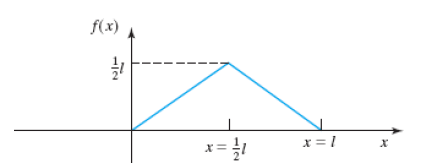
\includegraphics[width=0.6\textwidth]{figures/7.1.png}
        \caption{按箱中粒子函数展开的函数。}
        \label{fig:7.1}
    \end{figure}

    在(\ref{eq:7.33})中将$m$替换为$n$并带入到(\ref{eq:7.29})中,我们得到
    \begin{equation}
        f\left(x\right) = \sum_{n=1}^{\infty} \left[\int_{0}^{l} \psi_n^{\ast} f\left(x\right) \: \mathrm{d}x\right] \psi_n\left(x\right)
        \label{eq:7.34}
    \end{equation}
    这是任意函数 $f\left(x\right)$ 作为箱中粒子波函数 $\psi_n$ 的线性组合的展开所需的表达式。注意:定积分$\int_{0}^{l} \psi_n^{\ast} f\left(x\right) \: \mathrm{d}x$ 是一个数,而不是一个关于$x$的函数。

    我们现在使用(\ref{eq:7.29})来代表一个特定的函数,图(\ref{fig:7.1})所示的函数由下式定义:
    \begin{equation}
        \begin{cases}
            f\left(x\right) = 0, & 0 \leq x < \frac{l}{2} \\
            f\left(x\right) = 1, & \frac{l}{2} \leq x < l
        \end{cases}
        \label{eq:7.35}
    \end{equation}
    为了找到展开系数$a_n$,我们将(\ref{eq:7.35})和(\ref{eq:7.28})代入(\ref{eq:7.33})中:
    \begin{equation*}
        \begin{aligned}
            a_n &= \int_{0}^{l} \psi_n^{\ast} f\left(x\right) \: \mathrm{d}x = \left(\frac{2}{l}\right)^{1/2} \int_{0}^{l} \sin\left(\frac{n\pi x}{l}\right) f\left(x\right) \: \mathrm{d}x \\
            a_n &= \left(\frac{2}{l}\right)^{1/2} \int_{0}^{l/2} x\sin\left(\frac{n\pi x}{l}\right) \: \mathrm{d}x + \left(\frac{2}{l}\right)^{1/2} \int_{l/2}^{l} \left(l-x\right)\sin\left(\frac{n\pi x}{l}\right) \: \mathrm{d}x
        \end{aligned}
    \end{equation*}
    使用附录中的积分A.1,我们得到
    \begin{equation}
        a_n = \frac{\left(2l\right)^{3/2}}{n^2\pi^2}\sin\left(\frac{n\pi}{2}\right)
        \label{eq:7.36}
    \end{equation}
    将(\ref{eq:7.36})代入(\ref{eq:7.29}),我们得到[由于$\sin\left(n\pi/2\right)$在$n$为奇数时为1或-1,在$n$为偶数时为0]:
    \begin{equation*}
        f\left(x\right) = \frac{4l}{\pi^2}\left[\sin\left(\frac{\pi x}{l}\right) - \frac{1}{3^2}\sin\left(\frac{3\pi x}{l}\right) + \frac{1}{5^2}\sin\left(\frac{5\pi x}{l}\right) - \cdots\right]
    \end{equation*}
    \begin{equation}
        f\left(x\right) = \frac{4l}{\pi^2}\sum_{n=1}^{\infty}\left(-1\right)^{n+1}\frac{1}{\left(2n-1\right)^2}\sin\left[\left(2n-1\right)\frac{\pi x}{l}\right]
        \label{eq:7.37}
    \end{equation}
    其中$f\left(x\right)$由(\ref{eq:7.35})给出。让我们检查$x = \frac{1}{2}l$时(\ref{eq:7.37})的值:
    \begin{equation}
        f\left(\frac{l}{2}\right) = \frac{4l}{\pi^2}\left(1+\frac{1}{3^2}+\frac{1}{5^2}+\frac{1}{7^2}+\cdots\right)
        \label{eq:7.38}
    \end{equation}
    将 (\ref{eq:7.38}) 的右边作为我们在无穷级数中所取项数的函数列表,我们可以得到
    \begin{table}[h!]
        \centering
        \begin{tabular}{c|c|c|c|c|c|c|c}
            项数 & 1 & 2 & 3 & 4 & 5 & 20 & 100 \\
            \hline
            式(\ref{eq:7.38})的右侧 & $0.405l$ & $0.450l$ & $0.467l$ & $0.475l$ & $0.480l$ & $0.495l$ & $0.499l$
        \end{tabular}
    \end{table}
    \begin{figure}[h!]
        \centering
        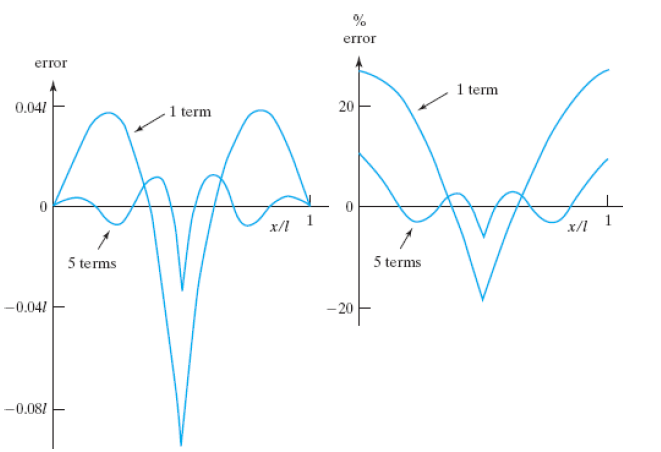
\includegraphics[width=0.6\textwidth]{figures/7.2.png}
        \caption{
            \centering
            \parbox{\linewidth}{
                \centering
                图 \ref{fig:7.1} 中以粒子箱中波函数展开的函数,展开式分别\\
                取 1 项和 5 项时,(a) 误差和(b) 百分比误差图。
            }
        }
        \label{fig:7.2}
    \end{figure}

    \noindent 如果我们取无穷多项,那么级数的和应为$\frac{1}{2}l$,与$f\left(\frac{l}{2}\right)$的值一致。假设级数成立,我们会得到一个有趣的结果,即(\ref{eq:7.38})中右侧括号的求和等于$\pi^2/8$。图7.2显示了$f\left(x\right) - \sum_{n-1}^{k}a_n\psi_n$的图形[其中$f$、$a_n$和$\psi_n$的定义见(\ref{eq:7.35})、(\ref{eq:7.36})和(\ref{eq:7.28})],其中$k$是取的项数,分别为1和5。随着 $k$(即展开式中的项数)的增加,级数逐渐趋近于 $f\left(x\right)$,而 $f$ 与级数之间的差值逐渐趋于零。

\subsection*{用本征函数展开函数}

     我们已经看到了用一组函数——箱中粒子能量本征函数——来展开一个函数的例子。我们可以使用许多不同的函数集来展开任意函数。如果每个品优函数 $f$ 都服从与 $g_i$ 函数相同的边界条件,并且可以根据以下条件展开为 $g_i$ 的线性组合,则称函数集 $g_1,g_2,\ldots,g_i,\ldots$ 为\textbf{完全集}(complete set):
    \begin{equation}
        f = \sum_{i}a_i g_i
        \label{eq:7.39}
    \end{equation}
    其中 $a_i$ 是常数。当然,我们很容易理解$f$和$g_i$都是同一组自变量的函数。(\ref{eq:7.39}) 中的和省略了极限。不言而喻,这个和包含了完整集合的所有成员。根据Fourier分析定理(我们尚未证明),可以证明粒子箱中的能量本征函数是一个完全集。

    我们现在假设:\textit{表示物理量的每个厄米算符的本征函数集是一个完全集。}(本征函数的完备性在很多情况下都可以证明,但在一般情况下必须假设。)因此,每个满足与本征函数集合相同边界条件的品优函数都可以根据 (\ref{eq:7.39}) 展开。方程 (\ref{eq:7.29}) 就是 (\ref{eq:7.39}) 的一个例子。

    谐振子波函数由厄米多项式$H_v$乘以一个指数因子给出[问题4.21c的式(4.86)]。根据展开公设,任何品优函数 $f\left(x\right)$ 都可以展开为谐振子能量本征函数的线性组合:
    \begin{equation*}
        f\left(x\right) = \sum_{n=0}^{\infty}a_n\left(2^nn!\right)^{-1/2}\left(\alpha/\pi\right)^{1/4}H_n\left(\alpha^{1/2}x\right)\mathrm{e}^{-\alpha x^2/2}
    \end{equation*}

    使用氢原子束缚态波函数来展开任意函数 $f\left(r,\theta,\phi\right)$如何?答案是这些函数并\textit{不}构成一个完全集,我们无法用它们来展开 $f$。要有一个完全集,我们必须使用特定厄米算符的\textit{所有}本征函数。除了氢原子哈密顿的束缚态本征函数外,我们还有与电离态相对应的连续态本征函数。如果将连续本征函数与束缚态本征函数一起包含在内,那么我们就得到了一个完全集。(对于箱中粒子和谐振子来说,连续函数不存在。)等式 (\ref{eq:7.39}) 意味着对连续本征函数(如果有的话)进行积分。因此,若$\psi_{nlm}\left(r,\theta,\phi\right)$是氢原子束缚态函数,$\psi_{Elm}\left(r,\theta,\phi\right)$是连续本征函数,则式(\ref{eq:7.39})变为
    \begin{equation*}
        f\left(r,\theta,\phi\right) = \sum_{n=1}^{\infty}\sum_{l=0}^{n-1}\sum_{m=-l}^{l}a_{nlm}\psi_{nlm}\left(r,\theta,\phi\right) + \sum_{l=0}^{\infty}\sum_{m=-l}^{l}\int_{0}^{\infty} a_{lm}\left(E\right) \psi_{Elm}\left(r,\theta,\phi\right) \:\mathrm{d}E
    \end{equation*}

    另一个例子:考虑算符$\hat{p}_x$的本征函数[式(\ref{eq:3.36})]:
    \begin{equation*}
        g_k = \mathrm{e}^{\mathrm{i}kx/\hbar}, \quad -\infty < k < \infty
    \end{equation*}
    这里的本征值都是连续的,任意函数 $f$ 的本征函数展开式(\ref{eq:7.39})变为
    \begin{equation*}
        f\left(x\right) = \int_{-\infty}^{\infty} a\left(k\right) \mathrm{e}^{\mathrm{i}kx/\hbar} \:\mathrm{d}k
    \end{equation*}
    具有良好数学基础的读者可能会发现,这个积分几乎就是 $a\left(k\right)$ 的Fourier变换。

    让我们对$f=\sum_{i}a_ig_i$ [式 (\ref{eq:7.39}) ] 中的展开系数进行计算,其中的 $g_i$ 函数是厄米算符的本征函数的完全集。这一过程与推导 (\ref{eq:7.33}) 所用的过程相同。我们将$f = \sum_{i}a_ig_i$与$g_k^{\ast}$相乘并对全空间积分:
    \begin{equation*}
        g_k^{\ast} f = \sum_{i} a_i g_k^{\ast} g_i
    \end{equation*}
    \begin{equation*}
        \int g_k^{\ast} f \:\mathrm{d}\tau = \sum_{i} a_i \int g_k^{\ast} g_i \:\mathrm{d}\tau = \sum_{i} a_i \delta_{ik} = a_k
    \end{equation*}
    \begin{equation}
        a_k = \int g_k^{\ast} f \:\mathrm{d}\tau
        \label{eq:7.40}
    \end{equation}
    其中我们用到了厄米算符本征函数之间的正交性:$\int g_k^{\ast} g_i \:\mathrm{d}\tau = \delta_{ik}$ [式 (\ref{eq:7.26}) ]。得出(\ref{eq:7.40})的过程会经常用到,值得记住。将(\ref{eq:7.40})中的$a_i$带入$f = \sum_{i}a_ig_i$中,我们得到
    \begin{equation}
        f = \sum_{i}\left[\int g_i^{\ast}f \:\mathrm{d}\tau\right]g_i = \sum_{i}\left\langle g_i \middle| f \right\rangle g_i
        \label{eq:7.41}
    \end{equation}

    \begin{examplebox}
        \textbf{例题:}令
        \begin{equation*}
            F\left(x\right) = \begin{cases}
                x\left(l-x\right), & 0 \leq x \leq l \\
                0, & \text{elsewhere}
            \end{cases}
        \end{equation*}
        将$F$用箱中粒子能量本征函数$\psi_n = \left(2/l\right)^{1/2}\sin\left(n\pi x/l\right), \: 0 \leq x \leq l$展开。
        \\
        
        注意到$F\left(0\right) = 0$以及$F\left(l\right) = 0$,因此满足与$\psi_n$相同的边界条件。我们可以使用$\psi_n$来展开$F$。展开式为$F = \sum_{n=1}^{\infty} a_n \psi_n$,其中系数$a_n = \int\psi_n^{\ast} F \:\mathrm{d}x$[式(\ref{eq:7.40})和(\ref{eq:7.39})]。因此,
        \begin{equation*}
            a_n = \int \psi_{n}^{\ast}F \:\mathrm{d}\tau = \left(\frac{2}{l}\right)^{1/2} \int_{0}^{l} \left(\sin\frac{n\pi x}{l}\right) x\left(l-x\right) \:\mathrm{d}x = \frac{2^{3/2}l^{5/2}}{n^3\pi^3}\left[1-\left(-1\right)^n\right]
        \end{equation*}
        其中积分计算的具体细节留作习题(问题7.18)。展开式$F = \sum_{n=1}^{\infty} a_n \psi_n$为
        \begin{equation*}
            x\left(l-x\right) = \frac{4l^2}{\pi^3}\sum_{n=1}^{\infty} \frac{1-\left(-1\right)^n}{n^3}\sin\left(\frac{n\pi x}{l}\right), \quad 0 \leq x \leq l
        \end{equation*}
        \\

        \textbf{练习:}令
        \begin{equation*}
            G\left(x\right) = \begin{cases}
                1, & 0 \leq x \leq l \\
                0, & \text{elsewhere}
            \end{cases}
        \end{equation*}
        将$G$用箱中粒子能量本征函数展开。由于 $G$ 在 原点和 $l$ 点不为零,因此展开式在这些点上不表示 $G$,而在其他地方表示 $G$。利用展开式的前 7 项非零项计算 $G$ 在$x = \frac{1}{4}l$处的值。使用前 70 个非零项重复上述步骤(使用可编程计算器)。(\textit{答案:}0.1219,0.9977.)
    \end{examplebox}

    以下是一条有用的定理:
    \begin{center}
        \parbox{0.8\textwidth}{
            \textbf{定理3:}令$g_1,g_2,\ldots$是厄米算符$\hat{A}$的本征函数完全集,令$F$是$\hat{A}$的本征函数,本征值为$k$(也就是说,$\hat{A}F = kF$)。若$F$展开为$F = \sum_{i}a_ig_i$,则展开式中的非零系数$a_i$仅对应于与$k$相同的本征值的本征函数$g_i$。(由于简并的存在,可能有多个本征函数$g_i$对应于同一本征值$k$。)
            
        }
    \end{center}

    因此,在 $F$ 的展开式中,我们只包括那些与 $F$ 具有相同本征值的本征函数。根据 $a_k = \int g_k^{\ast} f \:\mathrm{d}\tau$[公式 (\ref{eq:7.40}) ] 即可得出定理 3 的证明;若$F$和$g_i$对应于同一厄米算符$\hat{A}$的不同本征值,那它们是正交的[式(\ref{eq:7.22})],则$a_k$消失。

    我们偶尔会使用一种符号(称为 \textbf{ket} 符号),在这种符号中,函数 $f$ 用以下符号表示$\left| f \right\rangle$。这个符号似乎没有任何意义,但在量子力学的高级公式中,它具有特殊的意义。在ket符号中,式(\ref{eq:7.41})可以写成
    \begin{equation}
        \left| f \right\rangle = \sum_{i} \left| g_i\right\rangle \left\langle g_i \middle| f \right\rangle = \sum_i \left| i \right\rangle \left\langle i \middle| f \right\rangle
        \label{eq:7.42}
    \end{equation}
    Ket 符号方便地用于通过列出本征值来指定本征函数。例如,量子数分别为$n$、$l$和$m$的氢原子波函数可以写成$\psi_{nlm} = \left| n,l,m \right\rangle$。

    第\ref{sec:7.2 Hermitian Operators}和\ref{sec:7.3 Expansion in Terms of Eigenfunctions}节的内容可以总结为\textit{厄米算符的本征函数构成一个完整的正交集合,且本征值为实数。}

\section{对易算符的本征函数}
\label{sec:7.4 Eigenfunctions of Commuting Operators}
    如果态函数$\Psi$同时是两个算符$\hat{A}$和$\hat{B}$的本征函数,本征值分别为$a_j$和$b_j$,那么对物理量$A$的观测将得到值为$a_j$的结果,对物理量$B$的观测将得到值为$b_j$的结果。因此,当$\Psi$同时是$\hat{A}$和$\hat{B}$的本征函数时,物理量$A$和$B$都具有确定的值。

    在第 \ref{sec:5.1 Simultaneous Specification of Several Properties} 节中,我们对两个算符的同时本征函数做了一些说明。现在我们证明这些陈述。

    首先,我们证明:如果存在两个线性算符本征函数的共同\textit{完全集},那么这两个算符可对易。令$\hat{A}$和$\hat{B}$是两个线性算符,$g_1,g_2,\ldots$是共同的本征函数完全集:
    \begin{equation}
        \hat{A}g_i = a_ig_i, \quad \hat{B}g_i = b_ig_i
        \label{eq:7.43}
    \end{equation}
    其中$a_i$和$b_i$是本征值。我们需要证明
    \begin{equation}
        \left[\hat{A},\hat{B}\right] = 0
        \label{eq:7.44}
    \end{equation}
    方程(\ref{eq:7.44})是算符方程。要使两个算符相等,则用其中任何一个算符对任意品优函数 $f$ 运算的结果必须相同。因此我们必须证明
    \begin{equation*}
        \left(\hat{A}\hat{B} - \hat{B}\hat{A}\right)f = \hat{0}f = 0
    \end{equation*}
    其中$f$是任意函数。首先,我们根据完整的本征函数集$g_i$对 $f$ 进行展开(假设它遵守适当的边界条件):
    \begin{equation*}
        f = \sum_{i}c_i g_i
    \end{equation*}
    将算符$\hat{A}\hat{B}-\hat{B}\hat{A}$作用于上述方程,我们得到
    \begin{equation*}
        \left(\hat{A}\hat{B} - \hat{B}\hat{A}\right)f = \left(\hat{A}\hat{B} - \hat{B}\hat{A}\right)\sum_{i}c_ig_i
    \end{equation*}
    由于算符的积$\hat{A}\hat{B}$和$\hat{B}\hat{A}$是线性算符(问题3.16),我们有
    \begin{equation*}
        \left(\hat{A}\hat{B}-\hat{B}\hat{A}\right)f = \sum_{i}c_i\left(\hat{A}\hat{B}-\hat{B}\hat{A}\right)g_i = \sum_{i}\left[\hat{A}\left(\hat{B}g_i\right) - \hat{B}\left(\hat{A}g_i\right)\right]
    \end{equation*}
    其中用到了算符和与积的定义。使用本征值方程(\ref{eq:7.43}),我们得到
    \begin{equation*}
        \left(\hat{A}\hat{B}-\hat{B}\hat{A}\right)f = \sum_{i}\left[\hat{A}\left(b_ig_i\right)- \hat{B}\left(a_ig_i\right)\right] = \sum_{i}c_i\left(b_ia_ig_i - a_ib_ig_i\right) = 0
    \end{equation*}
    这就完成了如下定理的证明:
    \begin{center}
        \parbox{0.8\textwidth}{
            \textbf{定理4:}如果两个线性算符的本征函数完全集是相同的,那么这两个算符可对易。
        }
    \end{center}

    有时有人错误地认为:如果 $\hat{A}$ 和 $\hat{B}$ 存在一个共同的本征函数,那么它们就可对易。举一个例子可以说明这种说法是错误的,考虑球谐函数$Y_0^0$,它同时是$\hat{L}_z$和$\hat{L}_x$的本征函数,但显然这两个算符不可对易(第\ref{sec:5.3 Angular Momentum of a One-Particle System}节)。研究一下为这一错误说法提供的所谓证据是很有启发性的。令$g$为共同的本征函数:$\hat{A}g = ag$、$\hat{B}g = bg$。我们有
    \begin{equation*}
        \hat{A}\hat{B}g = \hat{A}bg = abg \quad \text{和} \quad \hat{B}\hat{A}g = \hat{B}ag = bag = abg
    \end{equation*}
    \begin{equation}
        \hat{A}\hat{B}g = \hat{B}\hat{A}g
        \label{eq:7.45}
    \end{equation}
    通过从式(\ref{eq:7.45})的两边消去$g$,我们完成了所谓的“证明”:
    \begin{equation}
        \hat{A}\hat{B} = \hat{B}\hat{A}\:(?)
        \label{eq:7.46}
    \end{equation}
    错误出现在从(\ref{eq:7.45})导出(\ref{eq:7.46})的过程中。$\hat{A}\hat{B}$和$\hat{B}\hat{A}$对单个函数$g$的作用结果是无法得出$\hat{A}\hat{B} = \hat{B}\hat{A}$的。(例如,当$\mathrm{d}/\mathrm{d}x$和$\mathrm{d}^2/\mathrm{d}x^2$作用于函数$\mathrm{e}^x$时,结果是相同的,但这并不意味着$\mathrm{d}/\mathrm{d}x$和$\mathrm{d}^2/\mathrm{d}x^2$是相等的。)这两个算符在作用于每个品优函数时必须得到相同的结果,我们才能得出它们相等的结论。因此,尽管$\hat{A}$和$\hat{B}$不可对易,但可能存在一个或更多的共同本征函数。然而,我们不可能有两个非对易算符的共同\textit{完整}本征函数集,正如我们在本节前面所证明的那样。

    我们已经证明了:若两个算符$\hat{A}$和$\hat{B}$的本征函数完全集是相同的,那么这两个算符可对易。现在我们证明:
    \begin{center}
        \parbox{0.8\textwidth}{
            \textbf{定理5:}如果两个厄米算符$\hat{A}$和$\hat{B}$可对易,我们可以为它们选择一组共同的完整本征函数。
        }
    \end{center}

    证明如下。令$g_i$和$a_i$分别是算符$\hat{A}$的本征函数和本征值:
    \begin{equation*}
        \hat{A}g_i = a_ig_i
    \end{equation*}
    将$\hat{B}$作用于上述方程,我们得到
    \begin{equation*}
        \hat{B}\hat{A}g_i = \hat{B}\left(a_ig_i\right)
    \end{equation*}
    由于$\hat{A}$和$\hat{B}$可对易,以及$\hat{B}$是线性算符,我们有
    \begin{equation}
        \hat{A}\left(\hat{B}g_i\right) = a_i\left(\hat{B}g_i\right)
        \label{eq:7.47}
    \end{equation}
    该方程表明:函数$\hat{B}g_i$也是算符$\hat{A}$的本征函数,本征值为$a_i$,与$g_i$一致。假设算符$\hat{A}$的本征值都是非简并的,那么对于任何给定的本征值$a_i$,存在唯一的线性无关的本征函数。如果是这样,那么两个对应于同一个本征值的本征函数$\hat{B}g_i$和$g_i$是线性相关的,也就是说,其中一个一定是另一个的简单乘积:
    \begin{equation}
        \hat{B}g_i = k_ig_i
        \label{eq:7.48}
    \end{equation}
    其中$k_i$是常数。这个方程说明了$g_i$是$\hat{B}$的本征函数,因此得证。在第 \ref{sec:7.3 Expansion in Terms of Eigenfunctions} 节中,我们假设任何表示物理量的算符的本征函数都构成一个完全集。因此,$g_i$构成一个完全集。

    我们刚才证明了非简并情况下的定理,那么简并情况下呢?设本征值$a_i$是$n$重简并的。由式(\ref{eq:7.47}),$\hat{B}g_i$也是$\hat{A}$的本征函数,本征值为$a_i$。因此,第\ref{sec:7.3 Expansion in Terms of Eigenfunctions}节中的定理3表明:若函数$\hat{B}g_i$可以用算符$\hat{A}$的本征函数完全集展开,那么除了本征值为$a_i$的项以外,其他项的系数均为零。也就是说,$\hat{B}g_i$一定是$n$个本征值为$a_i$的线性无关本征函数的线性组合:
    \begin{equation}
        \hat{B}g_i = \sum_{k=1}^{n}c_kg_k, \quad \text{其中} \quad \hat{A}g_k = a_ig_k \quad k = 1,2,\ldots,n
        \label{eq:7.49}
    \end{equation}
    其中$g_1,\ldots,g_n$表示$n$个本征值为$a_i$的算符$\hat{A}$的本征函数。式(\ref{eq:7.49})表明$g_i$不一定是$\hat{B}$的本征函数。然而,通过对$n$个对应于简并本征值$a_i$的线性无关的$\hat{A}$本征函数进行适当的线性组合,我们能构造出一组新的$n$个线性无关的本征函数,他们也将是$\hat{B}$的本征函数。该说法的证明见\textit{Merzbacher},第8.5节。

    因此,当$\hat{A}$和$\hat{B}$可对易时,我们可以为它们\textit{选择}一组共同的本征函数完全集。例如,考虑一个氢原子,我们已经证明了算符$\hat{L}_z$和$\hat{H}$是可对易的。如果我们愿意,我们可以将$\hat{B}$的本征函数中的$\phi$因子写成$\sin m\phi$和$\cos m\phi$的形式(第\ref{sec:6.6 The Bound-State Hydrogen-Atom Wave Functions}节)。如果这样做,除了 $m=0$ 的情况以外,我们就不会得到 $\hat{L}_z$ 的本征函数了。然而,根据\ref{sec:3.6 Degeneracy}节的定理,以下线性组合
    \begin{equation*}
        R\left(r\right)S\left(\theta\right)\left(\cos m\phi+\mathrm{i}\sin m\phi\right) = RS\mathrm{e}^{\mathrm{i}m\phi}, \quad m = -l,\ldots,l
    \end{equation*}
    给出的$\hat{L}_z$的本征函数仍然是$\hat{H}$的本征函数。

    将上述证明推广到两个以上算符的情况表明,当且仅当每个算符都与其他算符可对易时,对于一组厄米算符 $\hat{A},\hat{B},\hat{C},\ldots$,存在一个共同的完整本征函数集。

    与定理5相关的一个有用定理为:
    \begin{center}
        \parbox{0.8\textwidth}{
            \textbf{定理6:}若$g_m$和$g_n$是厄米算符$\hat{A}$的本征函数,但其本征值不同(即$\hat{A}g_m = a_mg_m$和$\hat{A}g_n = a_ng_n$,其中$a_m \neq a_n$),若线性算符$\hat{B}$与$\hat{A}$可对易,那么
            \begin{equation}
                \left\langle g_n \middle| \hat{B} \middle| g_m \right\rangle = 0, \quad a_n \neq a_m
                \label{eq:7.50}
            \end{equation}
        }
    \end{center}

    为了证明(\ref{eq:7.50}),我们从以下式子入手:
    \begin{equation}
        \left\langle g_n \middle| \hat{A}\hat{B} \middle| g_m \right\rangle = \left\langle g_n \middle| \hat{B}\hat{A} \middle| g_m \right\rangle
        \label{eq:7.51}
    \end{equation}
    对上式的左侧使用算符$\hat{A}$的厄米性质,有
    \begin{equation*}
        \begin{aligned}
            \left\langle g_n \middle| \hat{A}\hat{B} \middle| g_m \right\rangle = \left\langle g_n \middle| \hat{A} \middle| \hat{B} g_m \right\rangle = \left\langle \hat{B}g_m \middle| \hat{A} \middle| g_n \right\rangle^{\ast} &= \left\langle \hat{B}g_m \middle| a_n \middle| g_n \right\rangle^{\ast} \\
            &= a_n^{\ast}\left\langle g_n \middle| \hat{B}g_m \right\rangle = a_n\left\langle g_n \middle| \hat{B} \middle| g_m \right\rangle
        \end{aligned}
    \end{equation*}
    式(\ref{eq:7.51})的右侧可以写成
    \begin{equation*}
        \left\langle g_n \middle| \hat{B}\hat{A} \middle| g_m \right\rangle = \left\langle g_n \middle| \hat{B} \middle| \hat{A}g_m \right\rangle = a_m\left\langle g_n \middle| \hat{B} \middle| g_m \right\rangle
    \end{equation*}
    令(\ref{eq:7.51}) 左右两边的最终表达式相等,我们得到
    \begin{equation*}
        a_n \left\langle g_n \middle| \hat{B} \middle| g_m \right\rangle = a_m\left\langle g_n \middle| \hat{B} \middle| g_m \right\rangle
    \end{equation*}
    \begin{equation*}
        \left(a_n - a_m\right)\left\langle g_n \middle| \hat{B} \middle| g_m \right\rangle = 0
    \end{equation*}
    由于$a_n \neq a_m$,因此$\left\langle g_n \middle| \hat{B} \middle| g_m \right\rangle = 0$,这就证明了(\ref{eq:7.50})。

\section{宇称}
\label{sec:7.5 Parity}
    某些量子力学算符没有相对应的经典类似量。宇称算符就是一个例子。回想一下,谐振子的波函数要么是奇函数,要么是偶函数。我们将展示这一性质与宇称算符的关系。

    \textbf{宇称算符}(parity operator)$\hat{\Pi}$定义为其对任意函数$f$的以下作用结果:
    \begin{equation}
        \boxed{
            \hat{\Pi}f\left(x,y,z\right) = f\left(-x,-y,-z\right)
        }
        \label{eq:7.52}
    \end{equation}
    宇称算符将每个直角坐标替换为其负数。例如:$\hat{\Pi}\left(x^2 - z\mathrm{e}^{ay}\right) = x^2 + z\mathrm{e}^{-ay}$。

    与其他任意量子力学算符一样,我们对宇称算符的本征函数$g_i$和本征值$c_i$很感兴趣:
    \begin{equation}
        \hat{\Pi}g_i = c_ig_i
        \label{eq:7.53}
    \end{equation}
    问题的关键是求出$\hat{\Pi}$的平方:
    \begin{equation*}
        \hat{\Pi}^2f\left(x,y,z\right) = \hat{\Pi}\left[\hat{\Pi}f\left(x,y,z\right)\right] = \hat{\Pi}f\left[-x,-y,-z\right] = f\left(x,y,z\right)
    \end{equation*}
    由于$f$是任意给定的函数,我们得到$\hat{\Pi}^2$等于单位算符:
    \begin{equation}
        \hat{\Pi}^2 = \hat{1}
        \label{eq:7.54}
    \end{equation}
    
    我们现在将$\hat{\Pi}$作用到(\ref{eq:7.53})的两边,得到$\hat{\Pi}\hat{\Pi}g_i = \hat{\Pi}c_ig_i$。由于$\hat{\Pi}$是线性算符(问题7.26),我们有$\hat{\Pi}^2g_i = c_i\hat{\Pi}g_i$,则
    \begin{equation}
        \hat{\Pi}^2g_i = c_i^2g_i
        \label{eq:7.55}
    \end{equation}
    其中用到了本征方程(\ref{eq:7.53})。由于$\hat{\Pi}^2$是单位算符,式(\ref{eq:7.55})的左侧是$g_i$,那么
    \begin{equation*}
        g_i = c_i^2g_i
    \end{equation*}
    函数$g_i$不可能处处为零(根据物理原理,零总是被拒绝作为本征函数)。因此,两边除以$g_i$,我们得到$c_i^2 = 1$,即
    \begin{equation}
        c_i = \pm 1
        \label{eq:7.56}
    \end{equation}
    算符$\hat{\Pi}$的本征值为$+1$和$-1$。请注意,这一推导适用于其平方为单位算符的任何算符。

    本征方程$g_i$等于什么?本征方程(\ref{eq:7.53})为
    \begin{equation*}
        \hat{\Pi}g_i\left(x,y,z\right) = \pm g_i\left(x,y,z\right)
    \end{equation*}
    \begin{equation*}
        g_i\left(-x,-y,-z\right) = \pm g_i\left(x,y,z\right)
    \end{equation*}
    若本征值为$+1$,则$g_i\left(-x,-y,-z\right) = g_i\left(x,y,z\right)$,这表明$g_i$是偶函数;若本征值为$-1$,则$g_i\left(-x,-y,-z\right) = -g_i\left(x,y,z\right)$,这表明$g_i$是奇函数。因此,\textit{宇称算符$\hat{\Pi}$的本征函数为可能的品优奇函数和品优偶函数。}

    当宇称算符与哈密顿算符$\hat{H}$可对易时,根据第\ref{sec:7.4 Eigenfunctions of Commuting Operators}节的定理,我们可以为这两个算符选择一组共同的本征函数完全集。$\hat{H}$的本征函数是定态波函数$\psi_i$。因此,若
    \begin{equation}
        \left[\hat{\Pi}, \hat{H}\right] = 0
        \label{eq:7.57}
    \end{equation}
    波函数$\psi_i$可以被选择成为$\hat{\Pi}$的本征函数。我们刚刚证明了$\hat{\Pi}$的本征函数是奇函数或偶函数。因此,当(\ref{eq:7.57})成立时,每个波函数可以被选择为奇函数或偶函数。让我们看看宇称算符和哈密顿算符在什么情况下可对易。

    对于单粒子系统,我们有
    \begin{equation*}
        \left[\hat{H},\hat{\Pi}\right] = \left[\hat{T},\hat{\Pi}\right] + \left[\hat{V},\hat{\Pi}\right] = -\frac{\hbar^2}{2m}\left(\left[\frac{\partial^2}{\partial x^2},\hat{\Pi}\right] + \left[\frac{\partial^2}{\partial y^2},\hat{\Pi}\right] + \left[\frac{\partial^2}{\partial z^2},\hat{\Pi}\right]\right) + \left[\hat{V},\hat{\Pi}\right]
    \end{equation*}
    由于
    \begin{equation*}
        \begin{aligned}
            \hat{\Pi}\left[\frac{\partial^2}{\partial x^2}\left(x,y,z\right)\right] = \frac{\partial}{\partial\left(-x\right)}\frac{\partial}{\partial\left(-x\right)}f\left(-x,-y,-z\right) &= \frac{\partial^2}{\partial x^2}f\left(-x,-y,-z\right) \\
            &= \frac{\partial^2}{\partial x^2}\hat{\Pi}\left(x,y,z\right)
        \end{aligned}
    \end{equation*}
    其中$f$是任意函数,我们得到
    \begin{equation*}
        \left[\frac{\partial^2}{\partial x^2}, \hat{\Pi}\right] = 0
    \end{equation*}
    $y$和$z$坐标有类似的方程,则$\left[\hat{H},\hat{\Pi}\right]$变为
    \begin{equation}
        \left[\hat{H},\hat{\Pi}\right] = \left[\hat{V},\hat{\Pi}\right]
        \label{eq:7.58}
    \end{equation}
    现在
    \begin{equation}
        \hat{\Pi}\left[V\left(x,y,z\right)f\left(x,y,z\right)\right] = V\left(-x,-y,-z\right)f\left(-x,-y,-z\right)
        \label{eq:7.59}
    \end{equation}
    若势能函数为偶函数,即$V\left(-x,-y,-z\right) = V\left(x,y,z\right)$,则(\ref{eq:7.59})变为
    \begin{equation*}
        \hat{\Pi}\left[V\left(x,y,z\right)f\left(x,y,z\right)\right] = V\left(x,y,z\right)f\left(-x,-y,-z\right) = V\left(x,y,z\right)\hat{\Pi}f\left(x,y,z\right)
    \end{equation*}
    所以$\left[\hat{V},\hat{\Pi}\right] = 0$。因此,当势能函数为偶函数时,宇称算符和哈密顿算符可对易:
    \begin{equation}
        \left[\hat{H},\hat{\Pi}\right] = 0 \quad \text{若} V \text{为偶函数}
        \label{eq:7.60}
    \end{equation}

    这些结果很容易推广到 $n$ 粒子的情况。对于一个$n$粒子系统,宇称算符定义为
    \begin{equation}
        \hat{\Pi}f\left(x_1,y_1,z_1,\ldots,x_n,y_n,z_n\right) = f\left(-x_1,-y_1,-z_1,\ldots,-x_n,-y_n,-z_n\right)
        \label{eq:7.61}
    \end{equation}
    很容易发现,若$V$满足下式
    \begin{equation}
        V\left(x_1,y_1,z_1,\ldots,x_n,y_n,z_n\right) = V\left(-x_1,-y_1,-z_1,\ldots,-x_n,-y_n,-z_n\right)
        \label{eq:7.62}
    \end{equation}
    则(\ref{eq:7.57})成立。若$V$满足方程(\ref{eq:7.62}),则称其为$3n$坐标的\textbf{偶函数}(even function of the $3n$ coordinates)。总而言之,我们有
    \begin{center}
        \parbox{0.8\textwidth}{
            \textbf{定理7:}当势能 $V$ 是偶函数时,我们可以选择定态波函数,使每个波函数要么是偶函数,要么是奇函数。
        }
    \end{center}

    要么是偶数要么是奇数的函数被称为具有\textit{确定的宇称}(definite parity)。

    如果能级都是非简并能级(在一维问题中通常如此),那么每个能量本征值只对应一个独立的波函数,波函数中没有可选择的元素(除了任意的乘常数)。因此,对于非简并情况,当 $V$ 是偶函数时,定态波函数必须具有确定的宇称。例如,一维谐振子的势能函数为$V = \frac{1}{2}kx^2$,是偶函数,则波函数具有确定的宇称。

    氢原子势能函数是偶函数,类氢轨道可以选择具有确定的宇称(问题 7.22 和 7.29)。

    对于简并的情况,我们在波函数中有一个选择元素,因为与简并能级相对应的函数的任意线性组合是 $\hat{H}$ 的本征函数。对于简并能级,通过适当的线性组合,我们可以选择具有确定奇偶性的波函数,但并不要求它们必须具有确定的奇偶性。

    宇称有助于积分的计算。我们已经证明了当$f\left(x\right)$为奇函数时有$\int_{-\infty}^{\infty}f\left(x\right)\:\mathrm{d}x = 0$。让我们将这一结果推广到 $3n$ 维情况。$3n$ 个变量的\textbf{奇函数}(odd function)满足
    \begin{equation}
        g\left(-x_1,-y_1,-z_1,\ldots,-x_n,-y_n,-z_n\right) = -g\left(x_1,y_1,z_1,\ldots,x_n,y_n,z_n\right)
        \label{eq:7.63}
    \end{equation}
    若$g$是$3n$个变量的奇函数,则
    \begin{equation}
        \int_{-\infty}^{\infty}\cdots\int_{-\infty}^{\infty}g\left(x_1,\ldots,z_n\right)\:\mathrm{d}x_1\ldots\mathrm{d}z_n = 0
        \label{eq:7.64}
    \end{equation}
    其中的积分是对 $3n$ 个坐标的积分。这个等式成立的原因为:$\left(x_1,y_1,z_1,\ldots,x_n,y_n,z_n\right)$处$g$值对积分的贡献被$\left(-x_1,-y_1,-z_1,\ldots,-x_n,-y_n,-z_n\right)$处的$g$值抵消了。当积分是部分(但不一定是全部)变量的奇函数时,等式 (\ref{eq:7.64}) 也成立。参见问题 7.30 。

\section{测量和态叠加}
\label{sec:7.6 Measurement and the Superposition of States}
    量子力学可被视为一种计算测量各种可能结果概率的方法。例如,如果我们知道态函数$\Psi\left(x,t\right)$,那么在时刻$t$时测量粒子的位置位于$x$到$x+\mathrm{d}x$的无穷小区间内的概率为$\left|\Psi\left(x,t\right)\right|^2\mathrm{d}x$。现在,我们考虑对一般性质 $B$ 进行测量。我们的目的是找出如何使用 $\Psi$ 来计算 $B$ 的测量结果中每种可能结果的概率。本节的结果告诉我们状态函数 $\Psi$ 中包含哪些信息,是量子力学的核心所在。

    我们处理一个$n$粒子系统,使用$q$来表示$3n$个坐标。我们推测,算符 $\hat{B}$ 的本征值 $b_i$ 是对属性 $B$ 进行测量的唯一可能结果。使用$g_i$来表示$\hat{B}$的本征函数,我们有
    \begin{equation}
        \hat{B}g_i\left(q\right) = b_ig_i\left(q\right)
        \label{eq:7.65}
    \end{equation}

    我们在第 \ref{sec:7.3 Expansion in Terms of Eigenfunctions} 节中假设,任何代表物理可观测属性的厄米算符的本征函数都构成一个完全集。由于$g_i$构成一个完全集,我们可以将态函数 $\Psi$ 展开为
    \begin{equation}
        \Psi\left(q,t\right) = \sum_{i}c_i\left(t\right)g_i\left(q\right)
        \label{eq:7.66}
    \end{equation}
    为了允许$\Psi$随时间变化,我们在系数$c_i$中引入时间依赖性。

    由于$\left|\Psi\right|^2$表示概率密度,我们要求
    \begin{equation}
        \int\Psi^{\ast}\Psi \:\mathrm{d}\tau = 1
        \label{eq:7.67}
    \end{equation}
    将(\ref{eq:7.66})代入归一化条件,并使用式(\ref{eq:1.33 linear properties of complex conjugate })和(\ref{eq:1.32 properties of complex conjugate}),我们得到
    \begin{equation}
        1 = \int \sum_{i}c_i^{\ast}g_i^{\ast}\sum_ic_ig_i\:\mathrm{d}\tau = \int\sum_{i}c_i^{\ast}g_i^{\ast}\sum_kc_kg_k \:\mathrm{d}\tau = \int\sum_{i}\sum_{k}c_i^{\ast}c_k g_i^{\ast}g_k\:\mathrm{d}\tau
        \label{eq:7.68}
    \end{equation}

    由于 (\ref{eq:7.68}) 中两个和的求和下标不一定具有相同的值,因此这两个下标必须使用不同的符号。例如,考虑如下两个求和的积:
    \begin{equation*}
        \sum_{i=1}^{2}s_i\sum_{i=1}^{2}t_i = \left(s_1+s_2\right)\left(t_1+t_2\right) = s_1t_1 + s_1t_2 + s_2t_1 + s_2t_2
    \end{equation*}
    如果我们不小心写成了
    \begin{equation*}
        \sum_{i=1}^{2}s_i\sum_{i=1}^{2}t_i = \left(\text{错误的}\right)\sum_{i=1}^{2}\sum_{i=1}^{2}s_i t_i = \sum_{i=1}^{2}\left(s_1t_1+s_2t_2\right) = 2\left(s_1t_1+s_2t_2\right)
    \end{equation*}
    我们就得到了错误的答案。写乘积的正确方式是
    \begin{equation*}
        \sum_{i=1}^{2}s_i\sum_{i=1}^{2}t_i = \sum_{i=1}^{2}s_1\sum_{k=1}^{2}t_k = \sum_{i=1}^{2}\sum_{k=1}^{2}s_i t_k = \sum_{i=1}^{2}\left(s_it_1+s_it_2\right) = s_1t_1 + s_1t_2 + s_2t_1 + s_2t_2
    \end{equation*}
    这就得到了正确的结果。

    假定交换 (\ref{eq:7.68}) 中的无限求和与积分是成立的,我们得到
    \begin{equation*}
        \sum_{i}\sum_{k}c_i^{\ast}c_k\int g_i^{\ast}g_k\:\mathrm{d}\tau = 1
    \end{equation*}
    由于$\hat{B}$是厄米算符,它的本征函数之间应该是正交的[式(\ref{eq:7.26})];因此
    \begin{equation*}
        \sum_i\sum_kc_i^{\ast}c_k\delta_{ik} = 1
    \end{equation*}
    \begin{equation}
        \sum_i\left|c_i\right|^2 = 1
        \label{eq:7.69}
    \end{equation}
    我们很快就会指出 (\ref{eq:7.69}) 的重要性。

    回顾假设(第 \ref{sec:3.7 Average Values} 节),如果 $\Psi$ 是系统的归一化状态函数,那么属性 $B$ 的平均值为
    \begin{equation*}
        \left\langle B \right\rangle = \int \Psi^{\ast}\left(q,t\right)\hat{B}\Psi\left(q,t\right)\:\mathrm{d}\tau
    \end{equation*}
    将展开式(\ref{eq:7.66})代入上式,我们得到
    \begin{equation*}
        \left\langle B \right\rangle = \int\sum_{i}c_i^{\ast}g_i^{\ast}\hat{B}\sum_{k}c_kg_k\:\mathrm{d}\tau = \sum_{i}\sum_{k}c_i^{\ast}c_k\int g_i^{\ast}\hat{B}g_k\:\mathrm{d}\tau
    \end{equation*}
    其中我们用到了算符$\hat{B}$的线性性质。使用$\hat{B}g_k = b_kg_k$[式(\ref{eq:7.65})],我们有
    \begin{equation*}
        \left\langle B \right\rangle = \sum_{i}\sum_{k}c_i^{\ast}c_kb_k\int g_i^{\ast}g_k\:\mathrm{d}\tau = \sum_{i}\sum_{k}c_i^{\ast}c_kb_k\delta_{ik}
    \end{equation*}
    \begin{equation}
        \left\langle B \right\rangle = \sum_{i}\left|c_i\right|^2b_i
        \label{eq:7.70}
    \end{equation}

    我们如何解释 (\ref{eq:7.70}) ?我们在第 \ref{eq:3.39} 节中假设,当我们测量算符所代表的物理性质时,算符的本征值是我们能得到的唯一可能的数字。在对 $B$ 的任何测量中,我们都会得到其中一个值 $b_i$(假设没有实验误差)。现在回忆式(\ref{eq:3.81}):
    \begin{equation}
        \boxed{
            \left\langle B \right\rangle = \sum_{b_i}P\left(b_i\right)b_i
        }
        \label{eq:7.71}
    \end{equation}
    其中$P\left(b_i\right)$是对$B$进行测量,得到测量结果为$b_i$的概率。(\ref{eq:7.71}) 中的和涉及不同的本征值 $b_i$,而 (\ref{eq:7.70}) 中的和涉及不同的本征函数 $g_i$,因为展开式 (\ref{eq:7.66}) 涉及的是 $g_i$。如果每个本征值只有一个独立的本征函数,那么本征函数的总和就等于本征值的总和,比较 (\ref{eq:7.71}) 和 (\ref{eq:7.70}) 可以看出,当$\hat{B}$ 本征值没有简并时,$\left| c_i \right|^2$就是在测量属性 $B$ 时得到值 $b_i$ 的概率。请注意,这些值的总和为 1,因为概率的总和必定为1[式 (\ref{eq:7.69}) ]。假设本征值$b_i$是简并的。根据(\ref{eq:7.71}),$P\left(b_i\right)$由与$b_i$相乘的量给出。在简并的情况下,(\ref{eq:7.70})中有不止一项包含$b_i$,所以在测量中获得$b_i$的概率$P\left(b_i\right)$是所有本征值为$b_i$的本征函数对应的$\left| c_i \right|^2$的总和。我们已经证明了如下定理:
    \begin{center}
        \parbox{0.8\textwidth}{
            \textbf{定理8:}若$b_m$是算符$\hat{B}$的一个非简并本征值,$g_m$是对应的归一化本征函数($\hat{B}g_m = b_mg_m$),那么在量子力学系统中,测量时状态函数为$\Psi$时,对属性$B$的测量得到结果为$b_m$的概率由$\left| c_m \right|^2$给出,其中$c_m$是$g_m$在展开式$\Psi = \sum_{i}c_i g_i$中的系数。若$b_m$是简并本征值,则测量得到结果为$b_m$的概率由所有对应于$b_m$的本征函数的$\left| c_i \right|^2$的总和给出。
        }
    \end{center}

    什么时候可以准确预测 $B$ 的测量结果?若展开式$\Psi = \sum_{i}c_i g_i$ 中的系数 $c_i$ 全为零,除了$c_i$等于零,以及对于$ i \neq k$,$c_k \neq 0$的情况外,这是可以做到的。对于这种情况,式(\ref{eq:7.69})表明$\left|c_k\right|^2=1$,我们一定会得到值为$b_k$的结果。在该情况中,态函数$\Psi = \sum_ic_i g_i$简化为$\Psi = g_k$。当$\Psi$是$\hat{B}$的本征函数,本征值为$b_k$时,若我们对$B$进行测量,我们一定会得到值为$b_k$的结果。

    因此,我们可以将展开式$\Psi = \sum_{i}c_i g_i$[式(\ref{eq:7.66})]看作是将一般状态$\Psi$表达为算符$\hat{B}$本征态$g_i$的\textit{态叠加}(superposition)。每个本征态$g_i$对应于物理量$B$的一个可能测量结果$b_i$。任何本征函数$g_i$出现在$\Psi$展开式中的程度由$\left|c_i\right|^2$给出,它决定了在对$B$进行测量时得到结果$b_i$的概率。

    为了得到概率$\left|c_i\right|^2$,我们如何计算出展开系数$c_i$?我们将$g_j^{\ast}$与$\Psi = \sum_{i}c_i g_i$相乘,对全空间进行积分并使用厄米算符$\hat{B}$本征函数的正交性:
    \begin{equation*}
        \int g_j^{\ast}\Psi \: \mathrm{d}\tau = \sum_ic_i\int g_j^{\ast} g_i \: \mathrm{d}\tau = \sum_i c_i\delta_{ij}
    \end{equation*}
    \begin{equation}
        c_j = \int g_j^{\ast}\Psi \: \mathrm{d}\tau = \left\langle g_j \middle| \Psi \right\rangle
        \label{eq:7.72}
    \end{equation}

    在对性质$B$的测量中,发现非简并本征值$b_j$的概率为
    \begin{equation}
        \left|c_j\right|^2 = \left|\int g_j^{\ast}\Psi \: \mathrm{d}\tau\right|^2 = \left|\left\langle g_j \middle| \Psi \right\rangle\right|^2
        \label{eq:7.73}
    \end{equation}
    其中$\hat{B}g_j = b_jg_j$。量$\left\langle g_j \middle| \Psi \right\rangle$称为\textbf{概率幅}(probability amplitude)。

    因此,如果我们知道由状态函数 $\Psi$ 确定的系统状态,我们就可以使用 (\ref{eq:7.73}) 来预测对任何属性 $B$ 进行测量的各种可能结果的概率。确定 $\hat{B}$ 的本征函数 $g_j$ 和本征值 $b_j$ 是一个数学问题。

    为了在实验中确定测量 $B$ 时发现 $g_j$ 的概率,我们需要大量 $n$ 个相同的、无相互作用的系统,每个系统都处于相同的状态 $\Psi$,并测量每个系统中的属性 $B$。如果第$n_j$次测量得到的结果为$b_j$,则$P\left(b_j\right) = n_j/n = \left|\left\langle g_j \middle| \Psi \right\rangle\right|^2$。

    我们可以对定理 8 的第一部分进行如下重述:
    \begin{center}
        \parbox{0.8\textwidth}{
            \textbf{定理9:}若在某量子力学系统中对性质$B$进行测量,测量时的状态为$\Psi$,则观测到算符$\hat{B}$的非简并本征值$b_j$的概率为$\left|\left\langle g_j \middle| \Psi \right\rangle\right|^2$,其中$g_j$是已归一化的,对应于本征值$b_j$的本征函数。
        }
    \end{center}

    如果归一化函数 $g_j$ 和 $\Psi$ 非常相似,并且在空间的每个区域都有相似的大小,那么积分 $\left\langle g_j \middle| \Psi \right\rangle = \int g_j^{\ast}\Psi\:\mathrm{d}\tau$ 的绝对值就会很大。若$g_j$和$\Psi$不相似,那么在$g_i$很大而$\Psi$很小的区域中(反之亦然),乘积$g_j^{\ast}\Psi$就会很小,那么积分$\int g_j^{\ast}\Psi\:\mathrm{d}\tau$的绝对值也会很小,即找到$b_j$的概率$\left\langle g_j \middle| \Psi \right\rangle$也会很小。

    \begin{examplebox}
        \textbf{例题:}假设我们对氢原子核外电子的$L_z$分量进行测量,开始测量时系统的状态为$2p_x$。给出测量的可能结果,并给出每种结果的概率。使用这些概率计算$2p_x$状态的$\left\langle L_z \right\rangle$。
        \\

        由(\ref{eq:6.118}):
        \begin{equation*}
            \Psi = 2p_x = 2^{-1/2}\left(2p_1\right) + 2^{-1/2}\left(2p_{-1}\right)
        \end{equation*}
        这个方程将$\Psi$展开为$\hat{L}_z$的本征函数的线性组合。其中唯一两个具有非零系数的项为$2p_1$和$2p_{-1}$,它们的本征值分别为$\hbar$和$-\hbar$。(回想一下,1 和-1 的下标给出了量子数$m$,$\hat{L}_z$ 的本征值为 $m\hbar$。)使用定理8,我们取 $\Psi$ 展开式中系数绝对值的平方来得到概率。因此测量$L_z$时得到$\hbar$的概率为$\left|2^{-1/2}\right|^2 = 0.5$,得到$-\hbar$的概率也是$0.5$。为了从这些概率计算$\left\langle L_z \right\rangle$,我们使用(\ref{eq:7.71}):
        \begin{equation*}
            \left\langle L_z \right\rangle = \sum_{L_{z,i}}P\left(L_{z,i}\right)L_{z,i} = 0.5\hbar + 0.5\left(-\hbar\right) = 0
        \end{equation*}
        其中$P\left(L_{z,i}\right)$是测量时得到结果$L_{z,i}$的概率,除了两项以外,其他概率都为零。当然,$\left\langle L_z \right\rangle$也可以用平均值方程(\ref{eq:3.88})计算:$\left\langle 2p_x \middle| \hat{L}_z \middle| 2p_x \right\rangle$。
        \\

        \textbf{练习:}写出满足如下条件的氢原子波函数:对能量$E$测量时得到$n=2$能级的概率为1,对$L^2$测量时得到$2\hbar^2$的概率为1,对$L_z$测量时得到$-\hbar,0,\hbar$的概率相等。是否只有一种可能的答案?(\textit{部分答案:}否。)
    \end{examplebox}
    \begin{examplebox}
        \textbf{例题:}现有一个箱中粒子的系统,箱子长为$l$。对系统的能量进行一次测量,测量时粒子处于非定态$\Psi = 30^{1/2}l^{-5/2}x\left(l-x\right), \quad 0 \leq x \leq l$。给出测量的可能结果,并给出每种结果的概率。
        \\

        第 3.9 节的假设($c$)给出了可能的结果,即能量算符 $\hat{H}$ 的本征值。箱中粒子哈密顿算符的本征值为$E = n^2h^2/8ml^2$,其中$n = 1, 2, \ldots$,并且它们是非简并的。概率由$\Psi$对$\hat{H}$的本征函数的展开式给出。即$\Psi = \sum_{n=1}^{\infty}c_n\psi_n$,其中$\psi_n = \left(2/l\right)^{1/2}\sin\left(n\pi x/l\right)$。在(\ref{eq:7.41})之后的例子中,函数$x\left(l-x\right)$是根据箱中粒子能量本征函数展开的。状态函数$30^{1/2}l^{-5/2}x\left(l-x\right)$等于$x\left(l-x\right)$乘以归一化常数$30^{1/2}l^{-5/2}$。因此,因此,将前面例子中的系数乘以 $30^{1/2}l^{-5/2}$,就可以得到展开系数 $c_n$
        \begin{equation*}
            c_n = \frac{\left(240\right)^{1/2}}{n^3\pi^3}\left[1-\left(-1\right)^n\right]
        \end{equation*}
        观测到能量值$E_n = n^2h^2/8ml^2$的概率$P\left(E_n\right)$等于$\left|c_n\right|^2$:
        \begin{equation}
            P\left(E_n\right) = \frac{240}{n^6\pi^6}\left[1-\left(-1\right)^n\right]^2
            \label{eq:7.74}
        \end{equation}前几个可能值的概率为
        \vspace{1em}
        \begin{center}
            \renewcommand{\arraystretch}{1.5}
            \begin{tabular}{c|c|c|c|c|c}
                 $n$ & 1 & 2 & 3 & 4 & 5 \\
                \hline
                $E_n$ & $h^2/8ml^2$ & $4h^2/8ml^2$ & $9h^2/8ml^2$ & $16h^2/8ml^2$ & $25h^2/8ml^2$ \\
                \hline
                $P\left(E_n\right)$ & $0.99855$ & $0$ & $0.001370$ & $0$ & $0.000064$
            \end{tabular}
        \end{center}
        \vspace{1em}
        找到$n=1$能级的概率很高,这对应于抛物线态函数$30^{1/2}l^{-5/2}x\left(l-x\right)$与$n=1$的箱中粒子波函数$\left(2/l\right)^{1/2}\sin\left(\pi x/l\right)$非常相似(图\ref{fig:7.3})。零概率的能级为$n=2,4,6,\ldots$,这对应于以下事实:若原点与箱子的中心重合,则态函数$\Psi = 30^{1/2}l^{-5/2}x\left(l-x\right)$是偶函数,而$n=2,4,6,\ldots$的箱中粒子波函数是奇函数(图\ref{fig:2.3}),对$\Psi$的展开式没有贡献。当被积函数为奇函数时积分$\left\langle g_n \middle| \Psi \right\rangle$消失。
        \vspace{1em}
        \begin{center}
            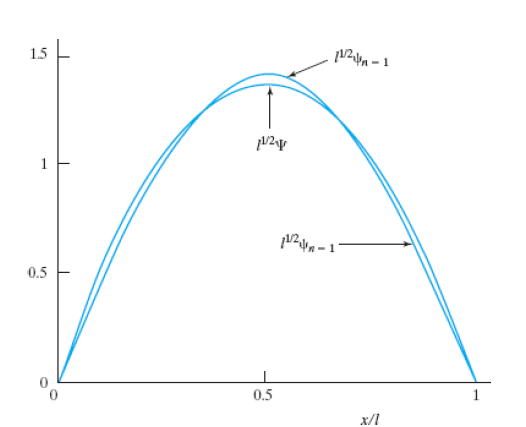
\includegraphics[width=0.5\textwidth]{Figures/7.3.png}
            \captionof{figure}{$\Psi = 30^{1/2}l^{-5/2}x\left(l-x\right)$和$n=1$箱中粒子波函数的图象}
            \label{fig:7.3}
        \end{center}
        \vspace{1em}
    \end{examplebox}

    若性质$B$的本征值可以连续变化(例如:位置,第\ref{sec:7.7 Position Eigenfunctions}节),则对$\Psi$展开式的求和(\ref{eq:7.66})变为对$b$所有可能值的积分:
    \begin{equation}
        \Psi = \int c_bg_b\left(q\right)\:\mathrm{d}b
        \label{eq:7.75}
    \end{equation}
    $\left| \left\langle g_b\left(q\right) \middle| \Psi \right\rangle \right|^2$依然是概率密度,也就是说,在位于$b$到$b+\mathrm{d}b$的无穷小区间内测量属性$B$时,得到结果$b$的概率为
    \begin{equation}
        \left| \left\langle g_b\left(q\right) \middle| \Psi\left(q,t\right) \right\rangle \right|^2\:\mathrm{d}b
        \label{eq:7.76}
    \end{equation}

\section{位置本征函数}
\label{sec:7.7 Position Eigenfunctions}
    我们推导出了线动量和角动量算符的本征函数。现在我们想知道:位置算符$\hat{x}$的本征函数是什么?

    算符$\hat{x}$表示对函数乘以$x$。将位置本征函数记作$g_a\left(x\right)$,写作
    \begin{equation}
        xg_a\left(x\right) = a g_a\left(x\right)
        \label{eq:7.77}
    \end{equation}
    其中的$a$代表可能的本征值。由此可见,
    \begin{equation}
        \left(x-a\right)g_a\left(x\right) = 0
        \label{eq:7.78}
    \end{equation}
    由(\ref{eq:7.78}),我们得知:
    \begin{equation}
        g_a\left(x\right) = 0, \quad \text{若} \quad x \neq a
        \label{eq:7.79}
    \end{equation}
    此外,由于本征函数处处为零是不可接受的,我们有
    \begin{equation}
        g_a\left(x\right) \neq 0, \quad \text{若} \quad x = a
        \label{eq:7.80}
    \end{equation}
    这些结论是有道理的。如果某状态函数是$\hat{x}$的本征函数,本征值为$a$,$\Psi = g_a\left(x\right)$,我们知道(第\ref{sec:7.6 Measurement and the Superposition of States}节):对$x$的测量一定得到值为$a$的结果。这只在$x \neq a$时有概率密度$\left|\Psi\right|^2$为零时才成立,与(\ref{eq:7.79})一致。

    在更进一步考虑$g_a\left(x\right)$的性质之前,我们先定义\textit{海维赛德阶梯函数}(Heaviside step function)(见图\ref{fig:7.4}):
    \begin{equation}
        \begin{aligned}
            H\left(x\right) & = 1, \quad x > 0 \\
            H\left(x\right) & = 0, \quad x < 0 \\
            H\left(x\right) & = \frac{1}{2}, \quad x = 0
        \end{aligned}
        \label{eq:7.81}
    \end{equation}
    \begin{figure}[h!]
        \centering
        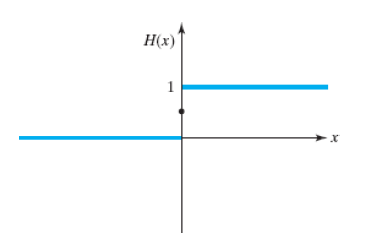
\includegraphics[width=0.4\textwidth]{Figures/7.4.png}
        \caption{海维赛德阶梯函数}
        \label{fig:7.4}
    \end{figure}

    接下来,我们再定义\textbf{狄拉克$\delta$函数}(Dirac $\delta$ function)$\delta\left(x\right)$为海维赛德阶梯函数的导数:
    \begin{equation}
        \delta\left(x\right) \equiv \frac{\mathrm{d}H\left(x\right)}{\mathrm{d}x}
        \label{eq:7.82}
    \end{equation}
    根据(\ref{eq:7.81})和(\ref{eq:7.82}),我们立即得出(另见图\ref{fig:7.4}):
    \begin{equation}
        \delta\left(x\right) = 0, \quad x \neq 0
        \label{eq:7.83}
    \end{equation}
    由于$H\left(x\right)$在$x=0$处的值突然变化,其导数在原点为无穷大:
    \begin{equation}
        \delta\left(x\right) = \infty, \quad x = 0
        \label{eq:7.84}
    \end{equation}

    我们可以通过设置 $x = t-a$,然后将符号 $t$ 改为 $x$,将这些方程稍作归纳。方程(\ref{eq:7.81})至(\ref{eq:7.84})可以写成
    \begin{equation}
        H\left(x-a\right) = 1, \quad x > a
        \label{eq:7.85}
    \end{equation}
    \begin{equation}
        H\left(x-a\right) = 0, \quad x < a
        \label{eq:7.86}
    \end{equation}
    \begin{equation}
        H\left(x-a\right) = \frac{1}{2}, \quad x = a
        \label{eq:7.87}
    \end{equation}
    \begin{equation}
        \delta\left(x-a\right) = \mathrm{d}H\left(x-a\right)/\mathrm{d}x
        \label{eq:7.88}
    \end{equation}
    \begin{equation}
        \delta\left(x-a\right) = 0, \quad x \neq a \quad \text{以及} \quad \delta\left(x-a\right) = \infty, \quad x = a
        \label{eq:7.89}
    \end{equation}

    现在,考虑如下的积分:
    \begin{equation*}
        \int_{-\infty}^{\infty}f\left(x\right)\delta\left(x-a\right)\:\mathrm{d}x
    \end{equation*}
    我们使用分部积分法计算:
    \begin{equation*}
        \int u \mathrm{d}v = uv - \int v \mathrm{d}u
    \end{equation*}
    \begin{equation*}
        u = f\left(x\right), \quad \mathrm{d}v = \delta\left(x-a\right)\:\mathrm{d}x
    \end{equation*}
    使用(\ref{eq:7.88}),我们有
    \begin{equation*}
        \mathrm{d}u = f'\left(x\right)\:\mathrm{d}x, \quad v = H\left(x-a\right)
    \end{equation*}
    \begin{equation*}
        \int_{-\infty}^{\infty}f\left(x\right)\delta\left(x-a\right)\:\mathrm{d}x = f\left(x\right)H\left(x-a\right)\bigg|_{-\infty}^{\infty} - \int_{-\infty}^{\infty}H\left(x-a\right)f'\left(x\right)\:\mathrm{d}x
    \end{equation*}
    \begin{equation}
        \int_{-\infty}^{\infty}f\left(x\right)\delta\left(x-a\right)\:\mathrm{d}x = f\left(\infty\right) - \int_{-\infty}^{\infty}H\left(x-a\right)f'\left(x\right)\:\mathrm{d}x
        \label{eq:7.90}
    \end{equation}
    其中,我们用到了(\ref{eq:7.85})和(\ref{eq:7.90})。由于$H\left(x-a\right)$在$x < a$时为零,(\ref{eq:7.90})变为
    \begin{equation*}
        \begin{aligned}
            \int_{-\infty}^{\infty}f\left(x\right)\delta\left(x-a\right)\:\mathrm{d}x & = f\left(\infty\right) - \int_{-\infty}^{a}H\left(x-a\right)f'\left(x\right)\:\mathrm{d}x \\
            & = \left.f\left(\infty\right) - \int_{-\infty}^{a}f'\left(x\right)\:\mathrm{d}x =  f\left(\infty\right) - f\left(x\right) \right|_{a}^{\infty}
        \end{aligned}
    \end{equation*}
    \begin{equation}
        \int_{-\infty}^{\infty}f\left(x\right)\delta\left(x-a\right)\:\mathrm{d}x = f\left(a\right)
        \label{eq:7.91}
    \end{equation}
    将(\ref{eq:7.91})与方程$\sum_{k}c_k\delta_{ik} = c_i$比较,我们可以看到,狄拉克$\delta$函数在积分中所起的作用与Kronecker三角在求和中所起的作用相同。(\ref{eq:7.91})的一个特例为$f\left(x\right) = 1$:
    \begin{equation*}
        \int_{-\infty}^{\infty}\delta\left(x-a\right)\:\mathrm{d}x = 1
    \end{equation*}

    狄拉克$\delta$函数的性质 (\ref{eq:7.89}) 与位置本征函数 $g_a\left(x\right)$ 的性质 (\ref{eq:7.79}) 和 (\ref{eq:7.80}) 一致。因此,我们暂定
    \begin{equation}
        g_a\left(x\right) = \delta\left(x-a\right)
        \label{eq:7.92}
    \end{equation}
    为了证明(\ref{eq:7.92}),我们现在需要证明其符合玻恩假设,即在$a$到$a+\mathrm{d}a$的无穷小区间内观测到$x$值的概率为$\left|\Psi\left(a,t\right)\right|^2\:\mathrm{d}a$。根据(\ref{eq:7.76}),这个概率由下式给出:
    \begin{equation}
        \left|\left\langle g_a\left(x\right) \middle| \Psi\left(x,t\right)\right\rangle\right|^2 \: \mathrm{d}a = \left|\int_{-\infty}^{\infty} g_a^{\ast}\left(x-\right)\Psi\left(x,t\right)\:\mathrm{d}x\right|^2 \: \mathrm{d}a
        \label{eq:7.93}
    \end{equation}
    先使用(\ref{eq:7.92})后使用(\ref{eq:7.91}),我们将(\ref{eq:7.93})变为
    \begin{equation*}
        \left|\int_{-\infty}^{\infty} \delta\left(x-a\right)\Psi\left(x,t\right)\:\mathrm{d}x\right|^2 \: \mathrm{d}a = \left|\Psi\left(a,t\right)\right|^2 \: \mathrm{d}a
    \end{equation*}
    得证。

    由于$\delta\left(x-a\right)$中的$a$可以去任何实数值,那么$\hat{x}$的本征值构成一个连续体:$-\infty < a < \infty$。与连续本征函数一致,$\delta\left(x-a\right)$不是平方可积的(问题7.43)。

    总而言之,位置的本征函数和本征值为
    \begin{equation}
        \hat{x}\delta\left(x-a\right) = a\delta\left(x-a\right)
        \label{eq:7.94}
    \end{equation}
    其中$a$是任意实数。

    $\delta$函数不是品优函数,因此我们所做的处理缺乏严谨性,会让数学家不寒而栗。不过,我们可以将$\delta$函数视为在原点处峰值逐渐增大的函数的极限情况,从而对其进行严格的表述(图 7.5)。 $\delta$函数其实不是函数,而是数学家所说的分布(distribution)。(见\url{en.wikipedia.org/wiki/Dirac_delta_function})
    \begin{figure}[h!]
        \centering
        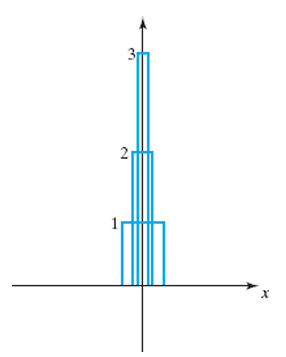
\includegraphics[width=0.3\textwidth]{Figures/7.5.png}
        \caption{近似 $\delta\left(x\right)$ 函数,精确度依次提高。每条曲线下的面积为 1。}
        \label{fig:7.5}
    \end{figure}

\section{量子力学的基本假设}
\label{sec:7.8 The Postulates of Quantum Mechanics}
    本节总结了前几章介绍的量子力学假设。

    \begin{center}
        \fbox{
            \parbox{\dimexpr\textwidth-3\fboxsep-3\fboxrule}{
            \textbf{假设1:}一个系统的状态由一个关于粒子坐标和时间的函数 $\Psi$ 给出。这个函数被称为状态函数或波函数,它包含了可以确定的关于系统的所有信息。我们进一步假设 $\Psi$ 是单值、连续和平方可积的。对于连续态,平方可积性的要求可以省略。
        }
    }
    \end{center}

    用 “波函数”来称呼 $\Psi$ 也许不是最好的选择。在三维空间中运动的物理波是三个空间坐标和时间的函数。然而,对于一个 $n$ 粒子系统,函数 $\Psi$ 是 $3n$ 空间坐标和时间的函数。因此,对于一个多粒子系统,我们不能把 $\Psi$ 解释为任何一种物理波。状态函数最好被视为一个函数,我们可以从中计算出系统的各种属性。$\Psi$所包含信息的性质是假设5及其结果的主题。

    \begin{center}
        \fbox{
            \parbox{\dimexpr\textwidth-3\fboxsep-3\fboxrule}{
            \textbf{假设2:}每个物理可观测属性都对应一个线性厄米算符。要找到这个算符,可以用笛卡尔坐标和相应的线动量分量写出可观测特性的经典力学表达式,然后用算符 $x \cdot$ 替换每个坐标 $x$,用算符 $-\mathrm{i}\hbar\ \partial/\partial x$ 替换每个动量分量 $p_x$.
        }
    }
    \end{center}

    我们在第 \ref{sec:7.2 Hermitian Operators} 节中看到,对厄米算符的限制源于物理量的平均值必须是实数的要求。线性的要求与第 \ref{sec:7.6 Measurement and the Superposition of States} 节讨论的态叠加密切相关。在我们对用 $\hat{B}$ 本征函数的叠加展开的状态其属性平均值 $B$ 的 (\ref{eq:7.70}) 的推导中,$\hat{B}$ 的线性性质起了关键作用。

    当经典量包含笛卡尔坐标与其共轭动量的乘积时,我们在构建正确的量子力学算符时就会遇到非对易的问题。已经提出了几种不同的规则来处理这种情况。见J. R. Shewell, \textit{Am. J. Phys.}, \textbf{27}, 16 (1959); E. H. Kerner and W. G. Sutcliffe, \textit{J. Math. Phys.}, \textbf{11}, 391 (1970); A. de Souza Dutra, \textit{J. Phys. A: Math. Gen.}, \textbf{39}, 203 (2006) (\url{arxiv.org/abs/0705.3247}).

    在非笛卡尔坐标中寻找量子力学算符的过程非常复杂。见K. Simon, \textit{Am. J. Phys.}, \textbf{33}, 60 (1965); G. R. Gruber, \textit{Found. Phys.}, \textbf{1} , 227 (1971).

    \begin{center}
        \fbox{
            \parbox{\dimexpr\textwidth-3\fboxsep-3\fboxrule}{
            \textbf{假设3:}对物理可观测属性 $B$ 的测量结果唯一可能的值是方程 $\hat{B}g_i = b_ig_i$ 中的本征值 $b_i$,其中 $\hat{B}$ 是与属性 $B$ 相对应的算符。本征函数 $g_i$ 必须是品优函数。
        }
    }
    \end{center}

    我们主要关注原子和分子的能级。它们由能量算符的本征值,即哈密顿量 $\hat{H}$ 给出。$\hat{H}$的本征方程,$\hat{H}\psi = E\psi$,是含时薛定谔方程。然而,要找到任何属性的可能值,都需要求解本征值方程。

    \begin{center}
        \fbox{
            \parbox{\dimexpr\textwidth-3\fboxsep-3\fboxrule}{
            \textbf{假设4:}若算符$\hat{B}$代表某个物理可观测量的线性厄米算符,那么其本征函数$g_i$构成一个完全集。
        }
    }
    \end{center}

    有些厄米算符的本征函数并不构成一个完全集(见\textit{Griffiths}, pp. 99, 106; \textit{Messiah}, p. 188; \textit{Ballentine}, Sec. 1.3)。完备性要求对于发展量子力学理论至关重要,因此有必要假设所有与可观测性质相对应的厄米算符都有一组完备的本征函数。假设 4 使我们能够将任何状态的波函数展开为任何量子力学算符的正交本征函数的叠加:
    \begin{equation}
        \Psi = \sum_{i}c_ig_i = \sum_{i}\left| g_i \right\rangle \left\langle g_i \middle| \Psi \right\rangle
        \label{eq:7.95}
    \end{equation}

    \begin{center}
        \fbox{
            \parbox{\dimexpr\textwidth-3\fboxsep-3\fboxrule}{
            \textbf{假设5:}若$\Psi\left(q,t\right)$表示$t$时刻系统的已归一化状态函数,那么$t$时刻物理可观测量$B$的平均值为
            \begin{equation}
                \boxed{
                    \left\langle B \right\rangle = \int \Psi^{\ast}\hat{B}\Psi\:\mathrm{d}\tau
                }
                \label{eq:7.96}
            \end{equation}
        }
    }
    \end{center}

    量子力学平均值的定义见第 \ref{sec:3.7 Average Values} 节,不应与经典力学中使用的时间平均值相混淆。

    根据假设4和5,我们已经在第\ref{sec:7.6 Measurement and the Superposition of States}节中得出了在对$B$的测量中观测到非简并本征值$b_i$的概率为$P\left(b_i\right) = \left|\int g_i^{\ast}\Psi \: \mathrm{d}\tau\right|^2 = \left|\left\langle g_i \middle| \Psi \right\rangle\right|^2$,其中$\hat{B}g_i = b_ig_i$。如果$\Psi$恰好是$\hat{B}$的本征函数直译,也就是说$\Psi = g_k$,那么$P\left(b_i\right)$变为$P\left(b_i\right) = \left|\int g_i^{\ast}g_k\:\mathrm{d}\tau\right|^2 = \left|\delta_{ik}\right|^2 = \delta_{ik}$,其中用到了厄米算符$\hat{B}$的本征函数之间互相正交的性质。当$\Psi = g_k$时,我们一定会得到$b_k$的测量结果。

    \begin{center}
        \fbox{
            \parbox{\dimexpr\textwidth-3\fboxsep-3\fboxrule}{
            \textbf{假设6:}未受干扰的量子力学系统状态的时间发展由含时薛定谔方程给出
            \begin{equation}
                \boxed{
                    -\frac{\hbar}{\mathrm{i}}\frac{\partial\Psi}{\partial t} = \hat{H}\Psi
                }
                \label{eq:7.97}
            \end{equation}
            其中$\hat{H}$是系统的哈密顿(也是能量)算符。
        }
    }
    \end{center}

    含时薛定谔方程关于时间的一阶微分方程,因此就像在经典力学中一样,未受干扰系统的当前状态决定了未来状态。然而,与经典力学中的状态知识不同,量子力学中的状态知识只涉及测量各种可能结果的\textit{概率}。 因此,假设我们有几个完全相同的非相互作用系统,每个系统在$t_0$时刻的状态函数均为$\Psi\left(t_0\right)$。 如果每个系统都不受干扰,那么每个系统的状态函数的变化都将遵循 (\ref{eq:7.97})。由于每个系统哈密顿量都相同,在未来的任意时刻$t_1$,每个系统的状态函数都将变为$\Psi\left(t_1\right)$。然而,假设我们在$t_2$时刻对每个系统的属性$B$进行一次观测。虽然在测量开始时,每个系统具有相同的态函数$\Psi\left(t_2\right)$,我们不会在每个系统中得到相同的结果。相反地,我们会得到一系列$b_i$的可能值,其中$b_i$是$\hat{B}$的本征值。 我们得到每个 $b_i$ 的相对次数可以通过下式计算:$\left|c_i\right|^2$,其中$\Psi\left(t_2\right) = \sum_{i}c_ig_i$,$g_i$是$\hat{B}$的本征函数。

    如果哈密顿算符与时间无关,我们就可能观测到具有确定能量$E$的状态。对于这样的状态,态函数必须满足
    \begin{equation}
        \hat{H}\Psi = E\Psi
        \label{eq:7.98}
    \end{equation}
    含时薛定谔方程变为
    \begin{equation*}
            -\frac{\hbar}{\mathrm{i}}\frac{\partial\Psi}{\partial t} = E\Psi
    \end{equation*}
    积分得到$\Psi = A\mathrm{e}^{-\mathrm{i}Et/\hbar}$,其中$A$是积分“常量”,与时间无关。函数$\Psi$与坐标和时间都相关,所以$A$是坐标的函数,我们将其命名为$\psi\left(q\right)$。因此,对于具有确定能量的状态,有
    \begin{equation}
        \Psi\left(q,t\right) = \mathrm{e}^{-\mathrm{i}Et/\hbar}\psi\left(q\right)
        \label{eq:7.99}
    \end{equation}
    函数$\psi\left(q\right)$满足定态薛定谔方程
    \begin{equation*}
        \hat{H}\psi\left(q\right) = E\psi\left(q\right)
    \end{equation*}
    由(\ref{eq:7.98})和(\ref{eq:7.99})可得上式。因子$\mathrm{e}^{-\mathrm{i}Et/\hbar}$只简单表明波函数$\Psi\left(q,t\right)$的相位随时间的变化,没有直接的物理意义。因此我们通常将$\psi\left(q\right)$视为“波函数”。哈密顿算符在量子力学中扮演着独特的角色,因为它出现在基本动力学方程——含时薛定谔方程中。$\hat{H}$的本征态(也成为定态)有特殊的性质,就是概率密度$\left|\Psi\right|^2$不随时间变化。

    含时薛定谔方程(\ref{eq:7.97})为$\left(\mathrm{i}\hbar \partial /\partial t - \hat{H}\right)\Psi = 0$。由于算符$\mathrm{i}\hbar \partial /\partial t - \hat{H}$是线性算符,那么含时薛定谔方程(\ref{eq:7.97})的解的任意线性组合也是(\ref{eq:7.97})的解。例如,若$\hat{H}$与时间无关,那么有定态解$\Psi_n = \mathrm{e}^{-\mathrm{i}E_nt/\hbar}\psi_n\left(q\right)$[式(\ref{eq:7.99})]。任意线性组合
    \begin{equation}
        \Psi = \sum_{n}c_n\Psi_n = \sum_{n}c_n\mathrm{e}^{-\mathrm{i}E_nt/\hbar}\psi_n\left(q\right)
        \label{eq:7.100}
    \end{equation}
    (其中$c_n$是与时间无关的常数)也是含时薛定谔方程的解,尽管它不是$\hat{H}$的本征函数。由于本征函数$\Psi_n$可以是复函数,若$\hat{H}$与时间无关,那么任何态函数都可以写成(\ref{eq:7.100})的形式。(另见第\ref{sec:9.8 Time-dependent Perturbation Theory}节。)状态函数 (\ref{eq:7.100}) 表示一种没有确定能量的状态。相反地,当我们测量能量时,得到能量值为$E_n$的概率为$\left|c_n\mathrm{e}^{-\mathrm{i}E_nt/\hbar}\right|^2 = \left|c_n\right|^2$。

    为了求出(\ref{eq:7.100})中的系数$c_n$,我们将(\ref{eq:7.100})在$t_0$时刻的表达式写成$\Psi\left(t_0\right) = \sum_{n}c_n\mathrm{e}^{-\mathrm{i}E_nt_0/\hbar}$\\$\psi_n\left(q\right)$。将其与$\psi_j^{\ast}\left(q\right)$相乘并对全空间进行积分,得到
    \begin{equation*}
        \left\langle \psi_j\left(q\right) \middle| \Psi\left(q,t_0\right) \right\rangle = \sum_{n}c_n\mathrm{e}^{-\mathrm{i}E_nt_0/\hbar}\left\langle \psi_j \middle| \psi_n \right\rangle = \sum_{n}c_n\mathrm{e}^{-\mathrm{i}E_nt_0/\hbar}\delta_{jn} = c_j\mathrm{e}^{-\mathrm{i}E_jt_0/\hbar}
    \end{equation*}
    则$c_n = \left\langle \psi_j \middle| \Psi\left(q,t_0\right) \right\rangle \mathrm{e}^{\mathrm{i}E_jt_0/\hbar}$。则(\ref{eq:7.100})变为
    \begin{equation}
        \Psi\left(q,t\right) = \sum_{n}\left\langle \psi_j \left(q\right) \middle| \Psi\left(q,t_0\right) \right\rangle \mathrm{e}^{-\mathrm{i}E_j\left(t-t_0\right)/\hbar}\psi_j\left(q\right), \quad \text{若}\hat{H}\text{与时间无关}
        \label{eq:7.101}
    \end{equation}
    其中$\hat{H}\psi_j = E_j\psi_j$,$\psi_j$被选择为正交的。方程 (\ref{eq:7.101}) 告诉我们如何从初始时间 $t_0$ 时的 $\Psi$ 求出时间 $t$ 时的 $\Psi$,当 $\hat{H}$ 与 $t$ 无关时,它是含时薛定谔方程的通解。[方程(\ref{eq:7.101})也可以直接从含时薛定谔方程导出,见问题7.46。]

    \begin{examplebox}
        \textbf{例题:}长度为$l$的一维势箱中有一粒子,其哈密顿量与时间无关,其态函数为$\Psi = 2^{-1/2}\psi_1+ $\\$ 2^{-1/2}\psi_2$,其中$\psi_1$和$\psi_2$分别是箱中粒子定态能量本征函数的$n=1$和$n=2$形式[式(\ref{eq:2.23 stationary state wave function for the particle in a box})]。(a)求出概率密度,表示为时间的函数;(b)证明$\left|\Psi\right|^2$振荡的周期为$T = 8ml^2/3h$;(c)使用Excel或Mathcad绘制$l\left|\Psi\right|^2$在每个时刻$jT/8$随$x/l$变化的图象,其中$j=0,1,2,\ldots,8$。
        \\

        (a)由于$\hat{H}$与时间无关,则在未来的任意时刻,$\Psi$的形式由(\ref{eq:7.100})给出,其中$c_1=2^{-1/2}$,$c_2=2^{-1/2}$,其他的$c$值全为零。因此,
        \begin{equation*}
            \begin{aligned}
                \Psi &= \frac{1}{\sqrt{2}}\mathrm{e}^{-\mathrm{i}E_1t/\hbar}\left(\frac{2}{l}\right)^{1/2}\sin\left(\frac{\pi x}{l}\right) + \frac{1}{\sqrt{2}}\mathrm{e}^{-\mathrm{i}E_2t/\hbar}\left(\frac{2}{l}\right)^{1/2}\sin\left(\frac{2\pi x}{l}\right) \\
                & = \frac{1}{\sqrt{2}}\mathrm{e}^{-\mathrm{i}E_1t/\hbar}\psi_1 + \frac{1}{\sqrt{2}}\mathrm{e}^{-\mathrm{i}E_2t/\hbar}\psi_2
            \end{aligned}
        \end{equation*}
        因此,我们有概率密度(见问题7.47)
        \begin{equation}
            \Psi^{\ast}\Psi = \frac{1}{2}\psi_1^2+\frac{1}{2}\psi_2^2 + \psi_1\psi_2\cos\left[\left(E_2-E_1\right)t/\hbar\right]
            \label{eq:7.102}
        \end{equation}

        (b)$\left|\Psi\right|^2$中与时间有关的因子为余弦因子(\ref{eq:7.102})。最小正周期为余弦函数的参数函数增加$2\pi$时的时间间隔,即$\left(E_2-E_1\right)T/\hbar = 2\pi$。由于$E_n = n^2h^2/8ml^2$,因此周期为$T = 2\pi\hbar/\left(E_2-E_1\right) = 8ml^2/3h$。

        (c)使用(\ref{eq:7.102})和$\psi_1$、$\psi_2$的表达式,以及$T = 2\pi\hbar/\left(E_2-E_1\right)$,我们有
        \begin{equation}
            l\left|\Psi\right|^2 = \sin^2\left(\pi x_r\right) + \sin^2\left(2\pi x_r\right) + \sin\left(\pi x_r\right)\sin\left(2\pi x_r\right)\cos\left(2\pi t/T\right)
            \label{eq:7.103}
        \end{equation}
        其中$x_r = x/l$。由于$t = jT/8$,对于每个$j$的值,函数图象很容易得到。图中显示,概率密度最大值在方框的左右两侧摆动。使用 Mathcad,我们可以制作出 $\left|\Psi\right|^2$ 随着时间变化而变化的影片(问题 7.47)。(\url{www.falstad.com/qm1d} 上有一个在线资源,可以让人们跟踪 $\left|\Psi\right|^2$ 作为时间函数的系统,例如箱中粒子或谐振子,对于任意选定的静止状态的初始混合物;人们可以通过点击底部的小圆圈并拖动圆圈内的每个旋转箭头来选择混合物。)
    \end{examplebox}

    当 $\hat{H}$ 与时间无关时,方程 (\ref{eq:7.100}) 是含时薛定谔方程的通解,其中的 $c_n$ 是常数。对于一个受到随时间变化的外力作用的系统来说,哈密顿算符包含一个与时间相关的项:$\hat{H} = \hat{H}^0 + \hat{H}^{\prime}\left(t\right)$,其中$\hat{H}^0$ 是系统在无外力作用下的哈密顿算符,$\hat{H}^{\prime}\left(t\right)$ 是系统与外力作用随时间变化的势能。在这种情况中,我们使用$\hat{H}^0$的定态本征函数来展开$\Psi$,与(\ref{eq:7.100})类似,除了$c_n$与时间$t$有关。例如,原子或分子暴露在电磁辐射(光)随时间变化的电场中;见第 \ref{sec:9.8 Time-dependent Perturbation Theory} 节。

    是什么决定了系统处于 (\ref{eq:7.99}) 这样的定态还是 (\ref{eq:7.100}) 这样的非定态?答案是系统的历史决定了它现在的状态。例如,如果我们将一个处于定态的系统暴露在辐射下,根据含时薛定谔方程,辐射会导致其状态转变为非定态;见第 \ref{sec:9.8 Time-dependent Perturbation Theory} 节。

    你可能会对玻恩假设的列表中没有 $\left|\Psi\left(x,t\right)\right|^2\:\mathrm{d}x$ 是在 $x$ 和 $x+\mathrm{d}x$ 之间找到粒子的概率感到奇怪。它是假设 5 的结果,我们现在就来说明这一点。方程(\ref{eq:3.81})为$\left\langle B \right\rangle = \sum_{b}P_bb$,其中$P_b$是测量具有离散值的属性$B$时观测到本征值$b$的概率。连续变量$x$对应的方程为$\left\langle x \right\rangle = \int_{-\infty}^{\infty}P\left(x\right)x\:\mathrm{d}x$,其中$P\left(x\right)$是测量连续变量$x$的概率密度。根据假设5,我们有$\left\langle x \right\rangle= \int_{-\infty}^{\infty}\Psi^{\ast}\hat{x}\Psi\:\mathrm{d}x = \int_{-\infty}^{\infty}\left|\Psi\right|^2x\:\mathrm{d}x$。将两个关于$\left\langle x \right\rangle$的表达式相比较,我们得到$\left|\Psi\right|^2$就是概率密度$P\left(x\right)$。

    第 \ref{chap:10} 章给出了涉及自旋和自旋统计定理的两个量子力学假设。

\section{测量和量子力学解释}
\label{sec:7.9 Measurement and the Interpretation of Quantum Mechanics}




















\section{矩阵}
\label{sec:7.10 Matrices}

\section*{总结}

\section*{习题}